\documentclass[9pt,twocolumn,twoside,lineno]{pnas-new}
% Use the lineno option to display guide line numbers if required.

\templatetype{pnasresearcharticle} % Choose template 
% {pnasresearcharticle} = Template for a two-column research article
% {pnasmathematics} %= Template for a one-column mathematics article
% {pnasinvited} %= Template for a PNAS invited submission

\title{City fingerprints: understanding city design through neighbourhood typologies}

% Use letters for affiliations, numbers to show equal authorship (if applicable) and to indicate the corresponding author
\author[a,1,2]{Kerry A. Nice}
\author[a,1]{Gideon D.P.A. Aschwanden} 
\author[a]{Jasper S. Wijnands}
\author[a]{Jason Thompson}
\author[a]{Haifeng Zhao}
\author[a,b]{Mark Stevenson}

\affil[a]{Transport, Health, and Urban Design Research Hub, Faculty of Architecture, Building, and Planning, University of Melbourne, Australia}
\affil[b]{Melbourne School of Engineering; and Melbourne School of Population and Global Health, University of Melbourne, Australia}

% Please give the surname of the lead author for the running footer
\leadauthor{Nice} 

% Please add a significance statement to explain the relevance of your work
% Authors must submit a 120-word maximum statement about the significance of their research paper written at a level understandable to an undergraduate educated scientist outside their field of speciality. The primary goal of the significance statement is to explain the relevance of the work in broad context to a broad readership. The significance statement appears in the paper itself and is required for all research papers.
\significancestatement{Knowledge about how cities work is urgently needed to minimise the negative impacts of rapid urbanization. We propose a unique method that uses block size and regularity derived from maps to assess differences in elements such as air pollution, infrastructure, and urban heat. By using these methods we can identify neighbourhoods and perform intra-city comparisons and thereby understand the distribution and composition of neighbourhood types across global cities. This approach allows identification of the characteristics and mixes of neighbourhoods in cities, an individual ‘fingerprint’, enabling lessons learned from high-performing cities to be applied across the world.}





% Please include corresponding author, author contribution and author declaration information
\authorcontributions{K.N. and G.A. developed the concept and designed experiments, analysed the results, and wrote the manuscript, J.W. and J.T. assisted with experiment design. All authors (including H.Z. and M.S.) discussed the results and implications and commented on the manuscript at all stages.}
\authordeclaration{The author(s) declare no competing interests.}
\equalauthors{\textsuperscript{1}K.N.(Kerry A. Nice) contributed equally to this work with G.A. (Gideon D.P.A. Aschwanden).}
\correspondingauthor{\textsuperscript{2}To whom correspondence should be addressed. E-mail: kerry.nice\@unimelb.edu.au}

% At least three keywords are required at submission. Please provide three to five keywords, separated by the pipe symbol.
\keywords{self organizing map $|$ city typologies $|$ neighborhood typologies $|$ urban morphology $|$ city science} 




\begin{abstract}
In the urban age, where the majority of the world's population live in cities, it is critical we improve our understanding of the strengths and limitations of existing city designs to ensure they are safe, clean, can deliver health co-benefits and importantly, are sustainable into the future. To enable this, a systematic and efficient means of performing inter- and intra-city comparisons based on urban form is urgently required. Until now, methods for comparing cities have been limited by scalability, often reliant upon non-standardised local input data that can be costly and difficult to obtain. To address this, we have developed a unique approach to determine the mix, distribution, and composition of neighbourhood types in cities based on dimensions of block size and regularity, sorted by a self-organising map. We illustrate the utility of the method to provide an understanding of the underlying city morphology by overlaying spatially standardised city metrics such as air pollution and transport activity across a set of 1667 global cities with populations exceeding 300,000. The approach reports associations between specific mixes of neighbourhood typologies and quantities of moving vehicles (r=0.97), impervious surfaces (r=0.86), and air pollution levels (aerosol optical depth r=0.58 and NO$_{2}$ r=0.57). This approach can identify the characteristics and neighbourhood mixes of well-performing urban areas while also producing city `fingerprints' that can be used to provide new metrics, insights, and drive improvements in city design now and into the future.
\end{abstract}

\dates{This manuscript was compiled on \today}
\doi{\url{www.pnas.org/cgi/doi/10.1073/pnas.XXXXXXXXXX}}

\begin{document}

\maketitle
\thispagestyle{firststyle}
\ifthenelse{\boolean{shortarticle}}{\ifthenelse{\boolean{singlecolumn}}{\abscontentformatted}{\abscontent}}{}

%% If your first paragraph (i.e. with the \dropcap) contains a list environment (quote, quotation, theorem, definition, enumerate, itemize...), the line after the list may have some extra indentation. If this is the case, add \parshape=0 to the end of the list environment.
%\dropcap{T}his PNAS journal template is provided to help you write your work in the correct journal format. Instructions for use are provided below. 
%
%Note: please start your introduction without including the word ``Introduction'' as a section heading (except for math articles in the Physical Sciences section); this heading is implied in the first paragraphs. 
%
%\section*{Guide to using this template on Overleaf}
%
%Please note that whilst this template provides a preview of the typeset manuscript for submission, to help in this preparation, it will not necessarily be the final publication layout. For more detailed information please see the \href{https://www.pnas.org/page/authors/format}{PNAS Information for Authors}.
%
%If you have a question while using this template on Overleaf, please use the help menu (``?'') on the top bar to search for \href{https://www.overleaf.com/help}{help and tutorials}. You can also \href{https://www.overleaf.com/contact}{contact the Overleaf support team} at any time with specific questions about your manuscript or feedback on the template.
%
%\subsection*{Author Affiliations}
%
%Include department, institution, and complete address, with the ZIP/postal code, for each author. Use lower case letters to match authors with institutions, as shown in the example. Authors with an ORCID ID may supply this information at submission.
%
%\subsection*{Submitting Manuscripts}
%
%All authors must submit their articles at \href{http://www.pnascentral.org/cgi-bin/main.plex}{PNAScentral}. If you are using Overleaf to write your article, you can use the ``Submit to PNAS'' option in the top bar of the editor window. 
%
%\subsection*{Format}
%
%Many authors find it useful to organize their manuscripts with the following order of sections;  title, author line and affiliations, keywords, abstract, significance statement, introduction, results, discussion, materials and methods, acknowledgments, and references. Other orders and headings are permitted.
%
%\subsection*{Manuscript Length}
%
%A standard 6-page article is approximately 4,000 words, 50 references, and 4 medium-size graphical elements (i.e., figures and tables). The preferred length of articles remains at 6 pages, but PNAS will allow articles up to a maximum of 12 pages.
%
%\subsection*{References}
%
%References should be cited in numerical order as they appear in text; this will be done automatically via bibtex, e.g. \cite{Ewing2010} and \cite{Ewing2010,Ewing2010}. All references cited in the main text should be included in the main manuscript file.
%
%\subsection*{Data Archival}
%
%PNAS must be able to archive the data essential to a published article. Where such archiving is not possible, deposition of data in public databases, such as GenBank, ArrayExpress, Protein Data Bank, Unidata, and others outlined in the \href{https://www.pnas.org/page/authors/journal-policies#xi}{Information for Authors}, is acceptable.
%
%\subsection*{Language-Editing Services}
%Prior to submission, authors who believe their manuscripts would benefit from professional editing are encouraged to use a language-editing service (see list at www.pnas.org/page/authors/language-editing). PNAS does not take responsibility for or endorse these services, and their use has no bearing on acceptance of a manuscript for publication. 
%
%\begin{figure}%[tbhp]
%\centering
%\includegraphics[width=.8\linewidth]{frog.png}
%\caption{Placeholder image of a frog with a long example legend to show justification setting.}
%\label{fig:frog}
%\end{figure}
%
%
%\begin{SCfigure*}[\sidecaptionrelwidth][t]
%\centering
%\includegraphics[width=11.4cm,height=11.4cm]{frog}
%\caption{This legend would be placed at the side of the figure, rather than below it.}\label{fig:side}
%\end{SCfigure*}
%
%\subsection*{Digital Figures}
%
%EPS, high-resolution PDF, and PowerPoint are preferred formats for figures that will be used in the main manuscript. Authors may submit PRC or U3D files for 3D images; these must be accompanied by 2D representations in TIFF, EPS, or high-resolution PDF format. Color images must be in RGB (red, green, blue) mode. Include the font files for any text.
%
%Images must be provided at final size, preferably 1 column width (8.7cm). Figures wider than 1 column should be sized to 11.4cm or 17.8cm wide. Numbers, letters, and symbols should be no smaller than 6 points (2mm) and no larger than 12 points (6mm) after reduction and must be consistent. 
%
%Figures and tables should be labelled and referenced in the standard way using the \verb|\label{}| and \verb|\ref{}| commands.
%
%Figure \ref{fig:frog} shows an example of how to insert a column-wide figure. To insert a figure wider than one column, please use the \verb|\begin{figure*}...\end{figure*}| environment. Figures wider than one column should be sized to 11.4 cm or 17.8 cm wide. Use \verb|\begin{SCfigure*}...\end{SCfigure*}| for a wide figure with side legends.
%
%\subsection*{Tables}
%Tables should be included in the main manuscript file and should not be uploaded separately.
%
%\subsection*{Single column equations}
%
%Authors may use 1- or 2-column equations in their article, according to their preference.
%
%To allow an equation to span both columns, use the \verb|\begin{figure*}...\end{figure*}| environment mentioned above for figures.
%
%Note that the use of the \verb|widetext| environment for equations is not recommended, and should not be used. 
%
%\begin{figure*}[bt!]
%\begin{align*}
%(x+y)^3&=(x+y)(x+y)^2\\
%       &=(x+y)(x^2+2xy+y^2) \numberthis \label{eqn:example} \\
%       &=x^3+3x^2y+3xy^3+x^3. 
%\end{align*}
%\end{figure*}
%
%
%\begin{table}%[tbhp]
%\centering
%\caption{Comparison of the fitted potential energy surfaces and ab initio benchmark electronic energy calculations}
%\begin{tabular}{lrrr}
%Species & CBS & CV & G3 \\
%\midrule
%1. Acetaldehyde & 0.0 & 0.0 & 0.0 \\
%2. Vinyl alcohol & 9.1 & 9.6 & 13.5 \\
%3. Hydroxyethylidene & 50.8 & 51.2 & 54.0\\
%\bottomrule
%\end{tabular}
%
%\addtabletext{nomenclature for the TSs refers to the numbered species in the table.}
%\end{table}
%
%\subsection*{Supporting Information Appendix (SI)}
%
%Authors should submit SI as a single separate SI Appendix PDF file, combining all text, figures, tables, movie legends, and SI references. PNAS will publish SI uncomposed, as the authors have provided it. Additional details can be found here: \href{https://www.pnas.org/page/authors/format#Supporting_Information}{policy on SI}. The PNAS Overleaf SI template can be found \href{https://www.overleaf.com/latex/templates/pnas-template-for-supplementary-information/wqfsfqwyjtsd}{here}. Refer to the SI Appendix in the manuscript at an appropriate point in the text. Number supporting figures and tables starting with S1, S2, etc.
%
%Authors who place detailed materials and methods in an SI Appendix must provide sufficient detail in the main text methods to enable a reader to follow the logic of the procedures and results and also must reference the SI methods. If a paper is fundamentally a study of a new method or technique, then the methods must be described completely in the main text.
%
%\subsubsection*{SI Datasets} 
%
%Supply .xlsx, .csv, .txt, .rtf, or .pdf files. This file type will be published in raw format and will not be edited or composed.
%
%
%\subsubsection*{SI Movies}
%
%Supply Audio Video Interleave (avi), Quicktime (mov), Windows Media (wmv), animated GIF (gif), or MPEG files. Movie legends should be included in the SI Appendix file. All movies should be submitted at the desired reproduction size and length. Movies should be no more than 10MB in size.
%
%
%\subsubsection*{3D Figures}
%
%Supply a composable U3D or PRC file so that it may be edited and composed. Authors may submit a PDF file but please note it will be published in raw format and will not be edited or composed.
%








Poorly managed urbanisation can impact urban residents through increased air pollution\cite{Stevenson2016,Sallis2016,Landrigan2017}, urban heat\cite{Coutts2012,Bowler2010}, urban sprawl\cite{Frank2000,Bettencourt2010}, and social isolation\cite{Vlahov2002}. In contrast, well managed urbanisation can promote economic activities and innovation, increase employment opportunities with economies of scale reducing the need for sprawling infrastructure\cite{Kuhnert2006,Bettencourt2007,Lobo2013}. For sustainable future cities, managing urbanisation processes so that they minimise the negative externalities and maximise the liveability, prosperity, and resilience of a city requires data and knowledge about how cities work. What is urgently needed therefore, is a systematic approach to compare cities that is a systematic method to identify different neighbourhoods within a city and to perform intra-city comparisons\cite{Louf2014a} to provide insights into i) the performance of cities at precinct or neighbourhood scales with respect to elements such as air pollution, infrastructure and urban heat and ii) what urban morphologies are best suited to the growing urban challenges of the 21st Century. To address this need, our framework allows us to compare a single element, as small as neighbourhoods of cities, across the globe, and to discover the mix and spatial distribution of different neighbourhood types in cities. We refer to this as an individual city `fingerprint'.

To discover how different cities work, research has been conducted through a number of methods to categorise cities and analyse underlying processes. Building on recent advances in computing power, artificial intelligence, and the wide availability of urban imagery, approaches have been created to discover unique characteristics of cities and how cities function. Large numbers of geo-tagged photos have been used to detect patterns of urban usage and public perception of a number of areas' functional and social attributes\cite{Liu2016,Zhou2014a}. Place Pulse, a database of urban imagery using crowd-sourced classifications (including safety, beauty, and liveliness) has attempted to quantify perceptions of urban areas\cite{Dubey2016,Naik2014} and inequality\cite{Salesses2013}. Doersch\cite{Doersch2012} used a large number of geo-localised street level images to discover common visual features across a number of cities. Enabled by remote sensing data, night-time light data has been used to categorise cities into stages of urbanisation and levels of economic activities\cite{Zhang2013}. Urban characteristics (road geometry, building dimensions and heights, and vegetation heights) have also been used to classify cities into typologies of differing periods of historical design and urban planning (i.e. 19th Century, 1950s, 1970s, etc.)\cite{Hermosilla2014}. 

Analysing the structural elements of road networks and urban blocks, generally the longest lasting part of an urban area, can provide clues as to the processes under which city development occurred (and currently continues)\cite{Porta2006a,Strano2012}. Road infrastructure can point to the dominant modes of transportation and governance systems underlying each urban area, with grid structures reflecting a top-down planning system\cite{Crouch1977,Courtat2011}, while T-shaped crossings point to more disorderly\cite{Jacobs1961} self-organised organic growth\cite{Cardillo2006}. Division of large land blocks (often originally agricultural land) can follow an evolutionary progression, either to medium sized manufacturing or smaller residential plots\cite{Fialkowski2008}. In addition, studies show that areas unconstrained by adjoining villages or topography are generally and most efficiently subdivided into smaller grids (i.e. regular rectangular plots)\cite{Strano2012}. The connection between the physical and topological structure of the road network in cities has parallels to the structural sociology field and transportation and economics. The `space syntax' community and Hillier\cite{Hillier1996} established a correlation between configurations of urban forms and variations of human interactions within it. 

Most of the methods described above require some amount of subjective classification of local input data; the quality and availability of which can vary widely when attempting to apply these methods to all types of cities world-wide, across multiple political districts. Existing empirical methods highlight underlying urban development mechanisms by evaluating the street network typology\cite{Hillier1989}, but this approach neglects their geometrical expanse and their function as places to stay. A method cannot rely solely on topology but needs to incorporate the urban geometry\cite{Louf2014a}.

Our unique method uses neighbourhood-level block size and regularity information to comprehensively explore the characteristics of cities across selected domains. The fundamental nature of city blocks, defined as the area bounded by surrounding streets, can be read as a simplified schematic view of the city\cite{Southworth2013}, highlighting both the structure and organisation of the city, as well as the process of the urban development and morphology. This makes the city block the most used and accessible urban element for urban analysis and basic common elements in city design typologies and theory\cite{Jacobs1961,Ewing2010,Louf2014a}. Blending theory with globally available datasets at scale can enable new insights into the form and function of the world's cities. This method allows us to find the mix of commonalities and unique elements, a `fingerprint' of each city, to understand what works and doesn't work in a city, an understanding essential to best manage the world's rapid urbanisation for health and well-being.

\section*{Results}


The methodology we present uses data on land use and block size extracted from maps and deploys a Self Organising Map (SOM) algorithm to organise them. SOM is an unsupervised sorting algorithm that iteratively sorts a list of vectors (containing higher dimensional information), projecting them into lower dimensions, adding a spatial component by moving similar vectors closer and spreading dissimilar vectors further away.

We demonstrate the method using information derived from 300$\times$300m map segments of 1.7 million locations sampled from the world's largest cities (populations greater than 300,000). The results are a 2-dimensional map of clusters of neighbourhood types seen in the 1667 cities where 2.2 billion people currently live. Figure \ref{fig:somresults} shows a visualisation of the results of this process. Each (x,y) node location in the SOM can contain either zero maps (and is shown in black) or a single or many maps (and is represented by one of the maps). A colour scheme map (Figure \ref{fig:colormap}) is used to convert the (x,y) locations into red/green/blue (RGB) values to plot the spatial distributions of neighbourhood types in Tokyo and New York, for example, see Figures \ref{fig:citylocations}a and \ref{fig:citylocations}b. Visualisations of the SOM showing only locations in Tokyo and New York are shown in Figures \ref{fig:citylocations}c and \ref{fig:citylocations}d. Red Boxes and Lines (i, ii, iii, and iv) in Figure \ref{fig:citylocations} connects some example spatial regions in these cities to their corresponding neighbourhood types.

\begin{figure*}
%\begin{figure}
\centering
%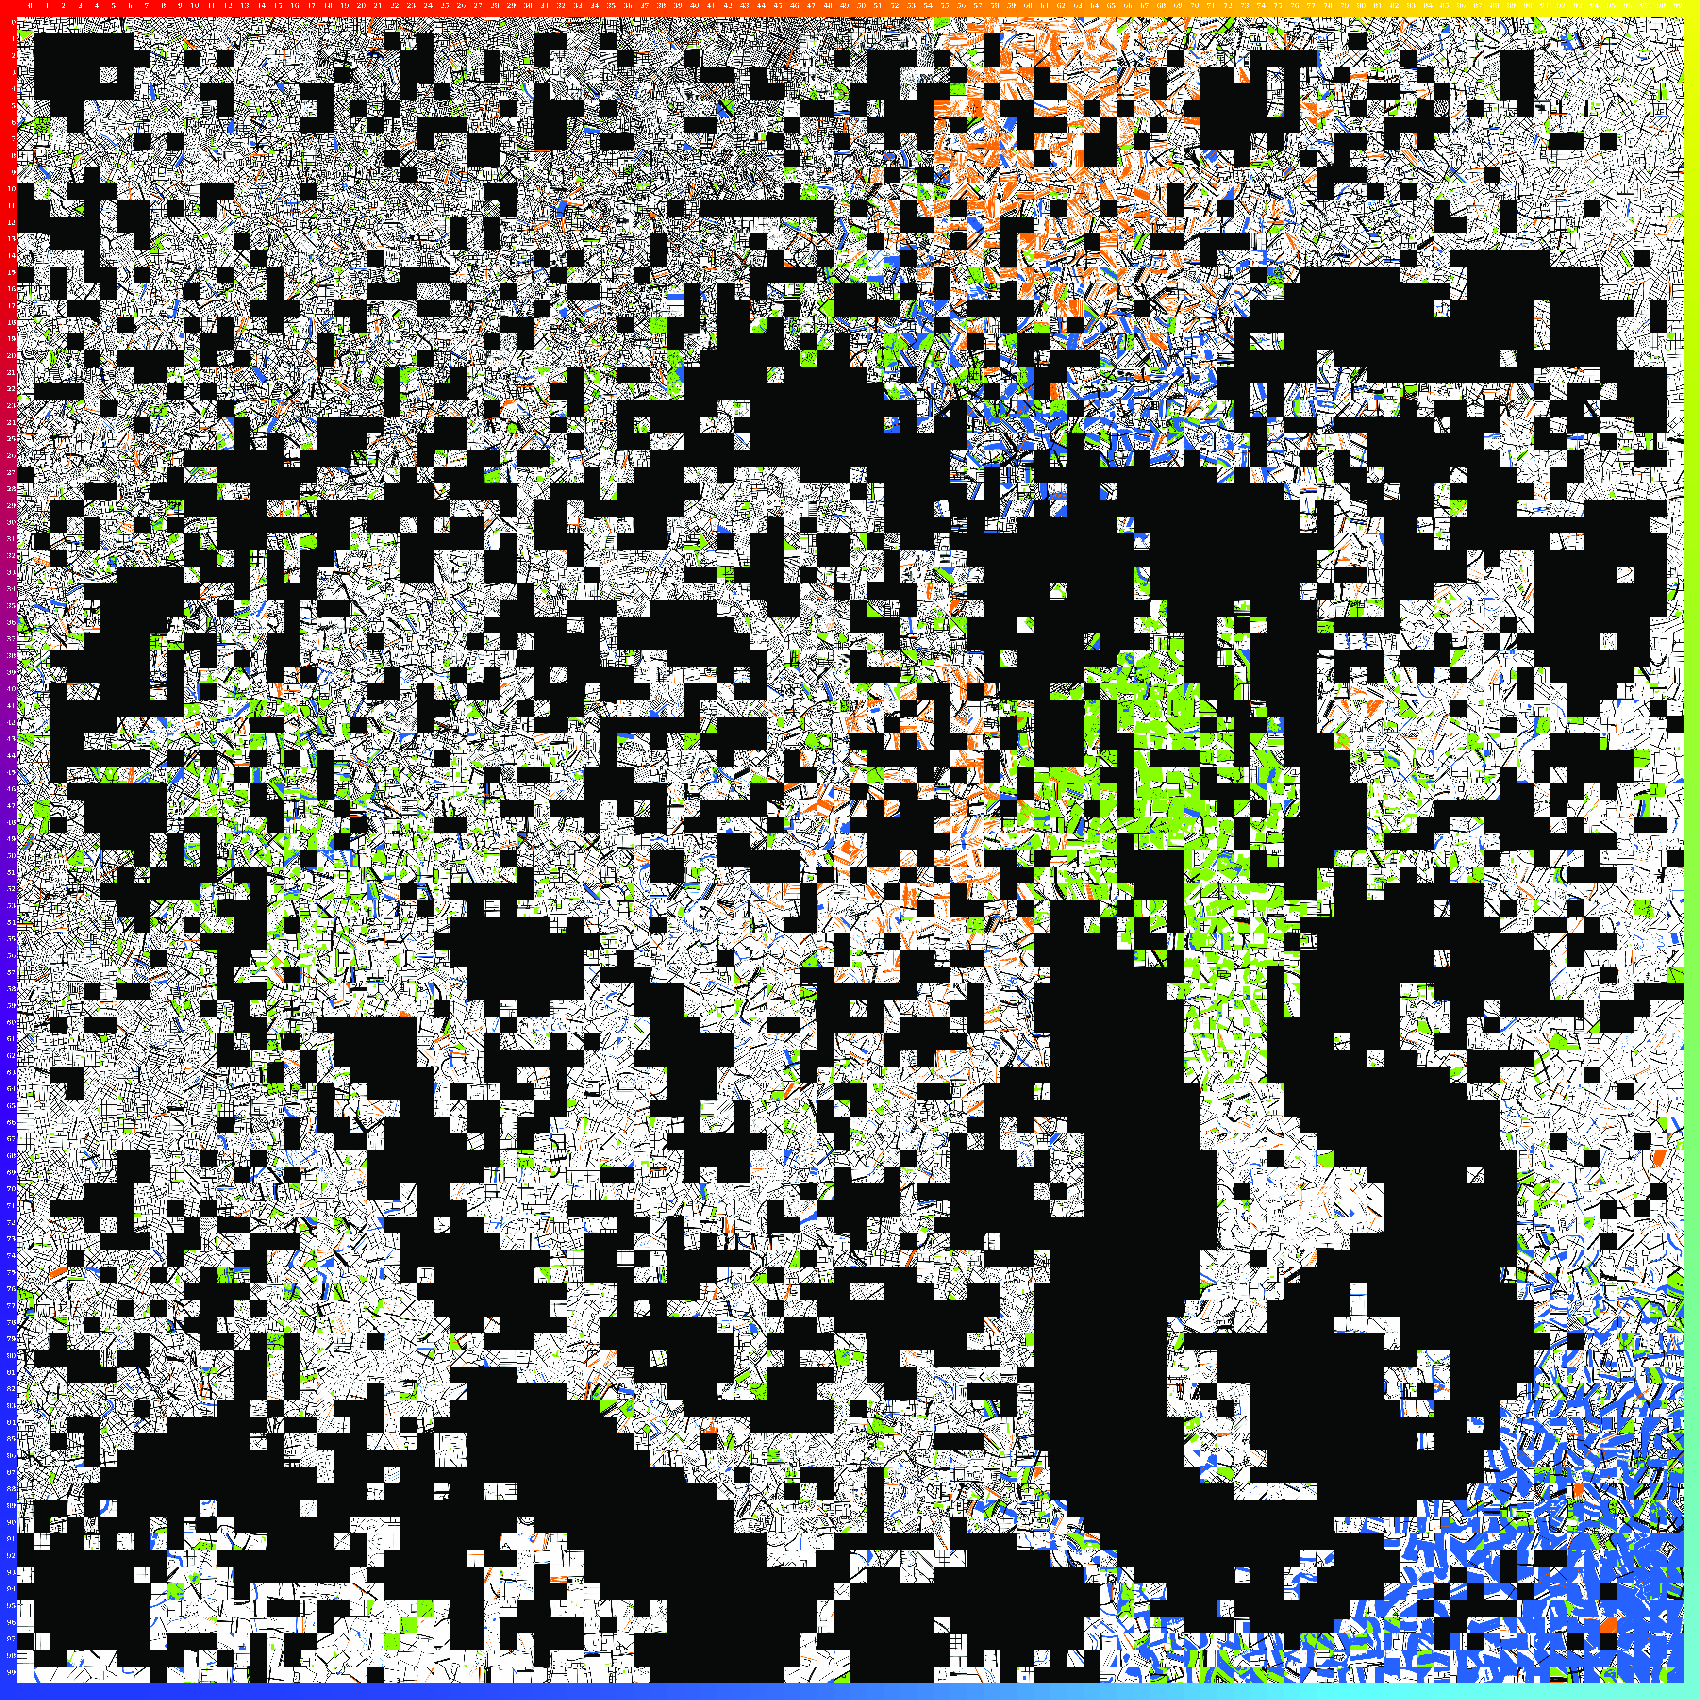
\includegraphics[trim={0 0 0 0},clip,scale=0.15]{BlockTypologies_Figures2-0.png}
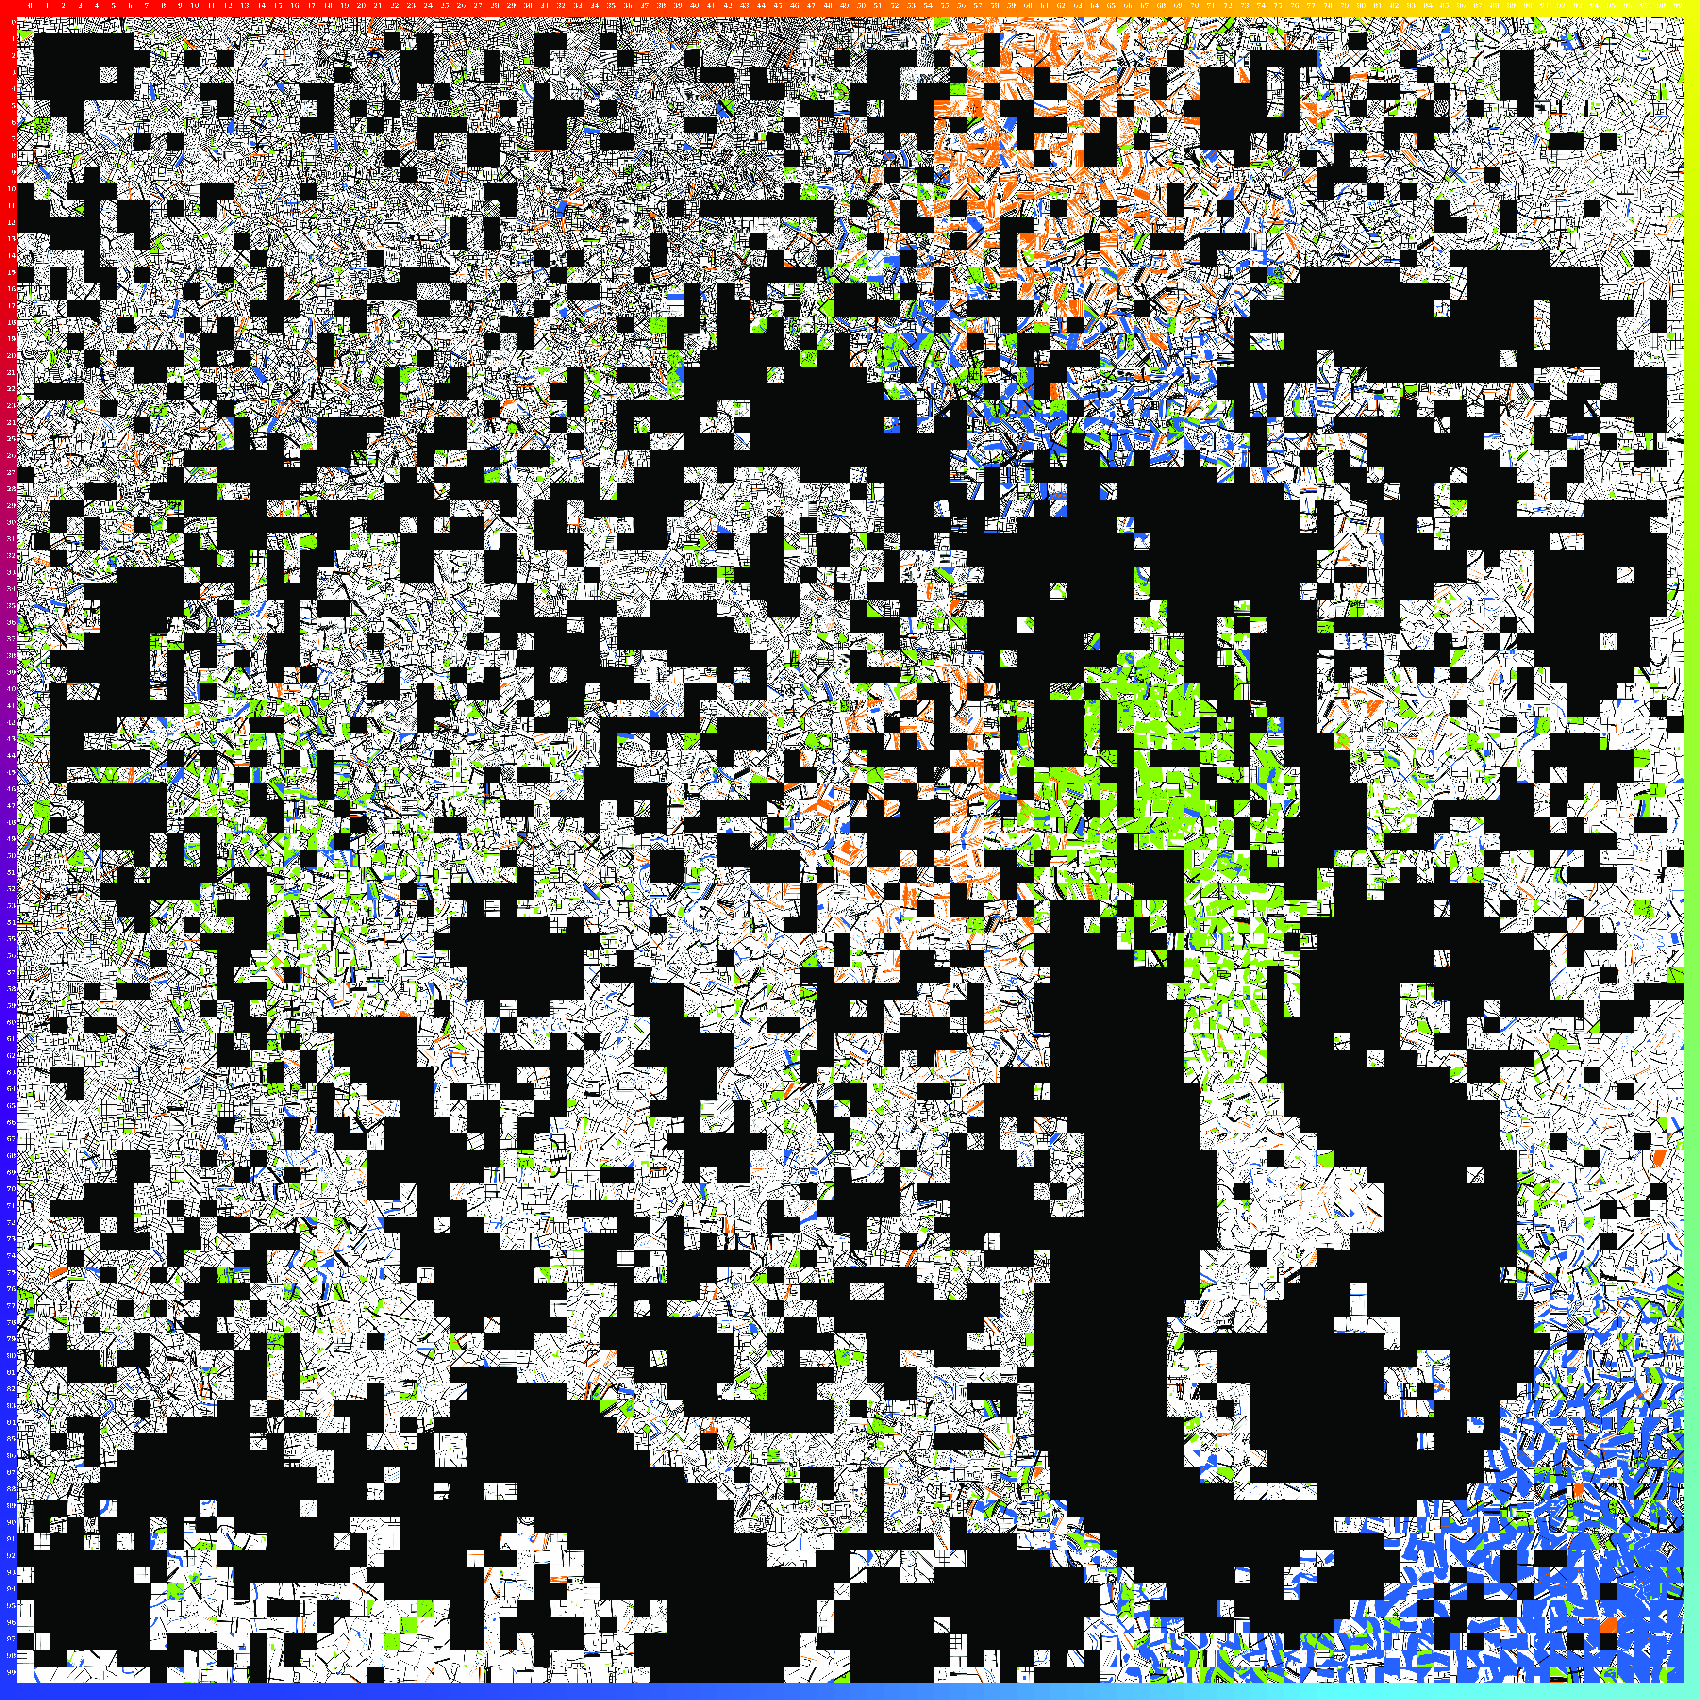
\includegraphics[width=.5\linewidth]{BlockTypologies_Figures2-0.png}
\caption{\bf A visualisation of the 2-dimensional 100$\times$100 SOM trained with 1.7 million map images from 1667 cities. Each (x,y) point shows a representative image associated with each node while nodes without associated images are shown in black. Border shows colour coding scheme (Figure \ref{fig:colormap}) for SOM (x,y) locations used in Figure \ref{fig:citylocations}.}
 \label{fig:somresults}
%\end{figure} 
\end{figure*}

\begin{figure}
\centering

\includegraphics[trim={0 0 0 0},clip,scale=0.09]{cubediagonal.png}
\caption{\bf Colour map used to plot SOM (x,y) locations in Figure \ref{fig:citylocations}. }
 \label{fig:colormap}
\end{figure} 

\begin{figure*}
\centering
%\frame{
%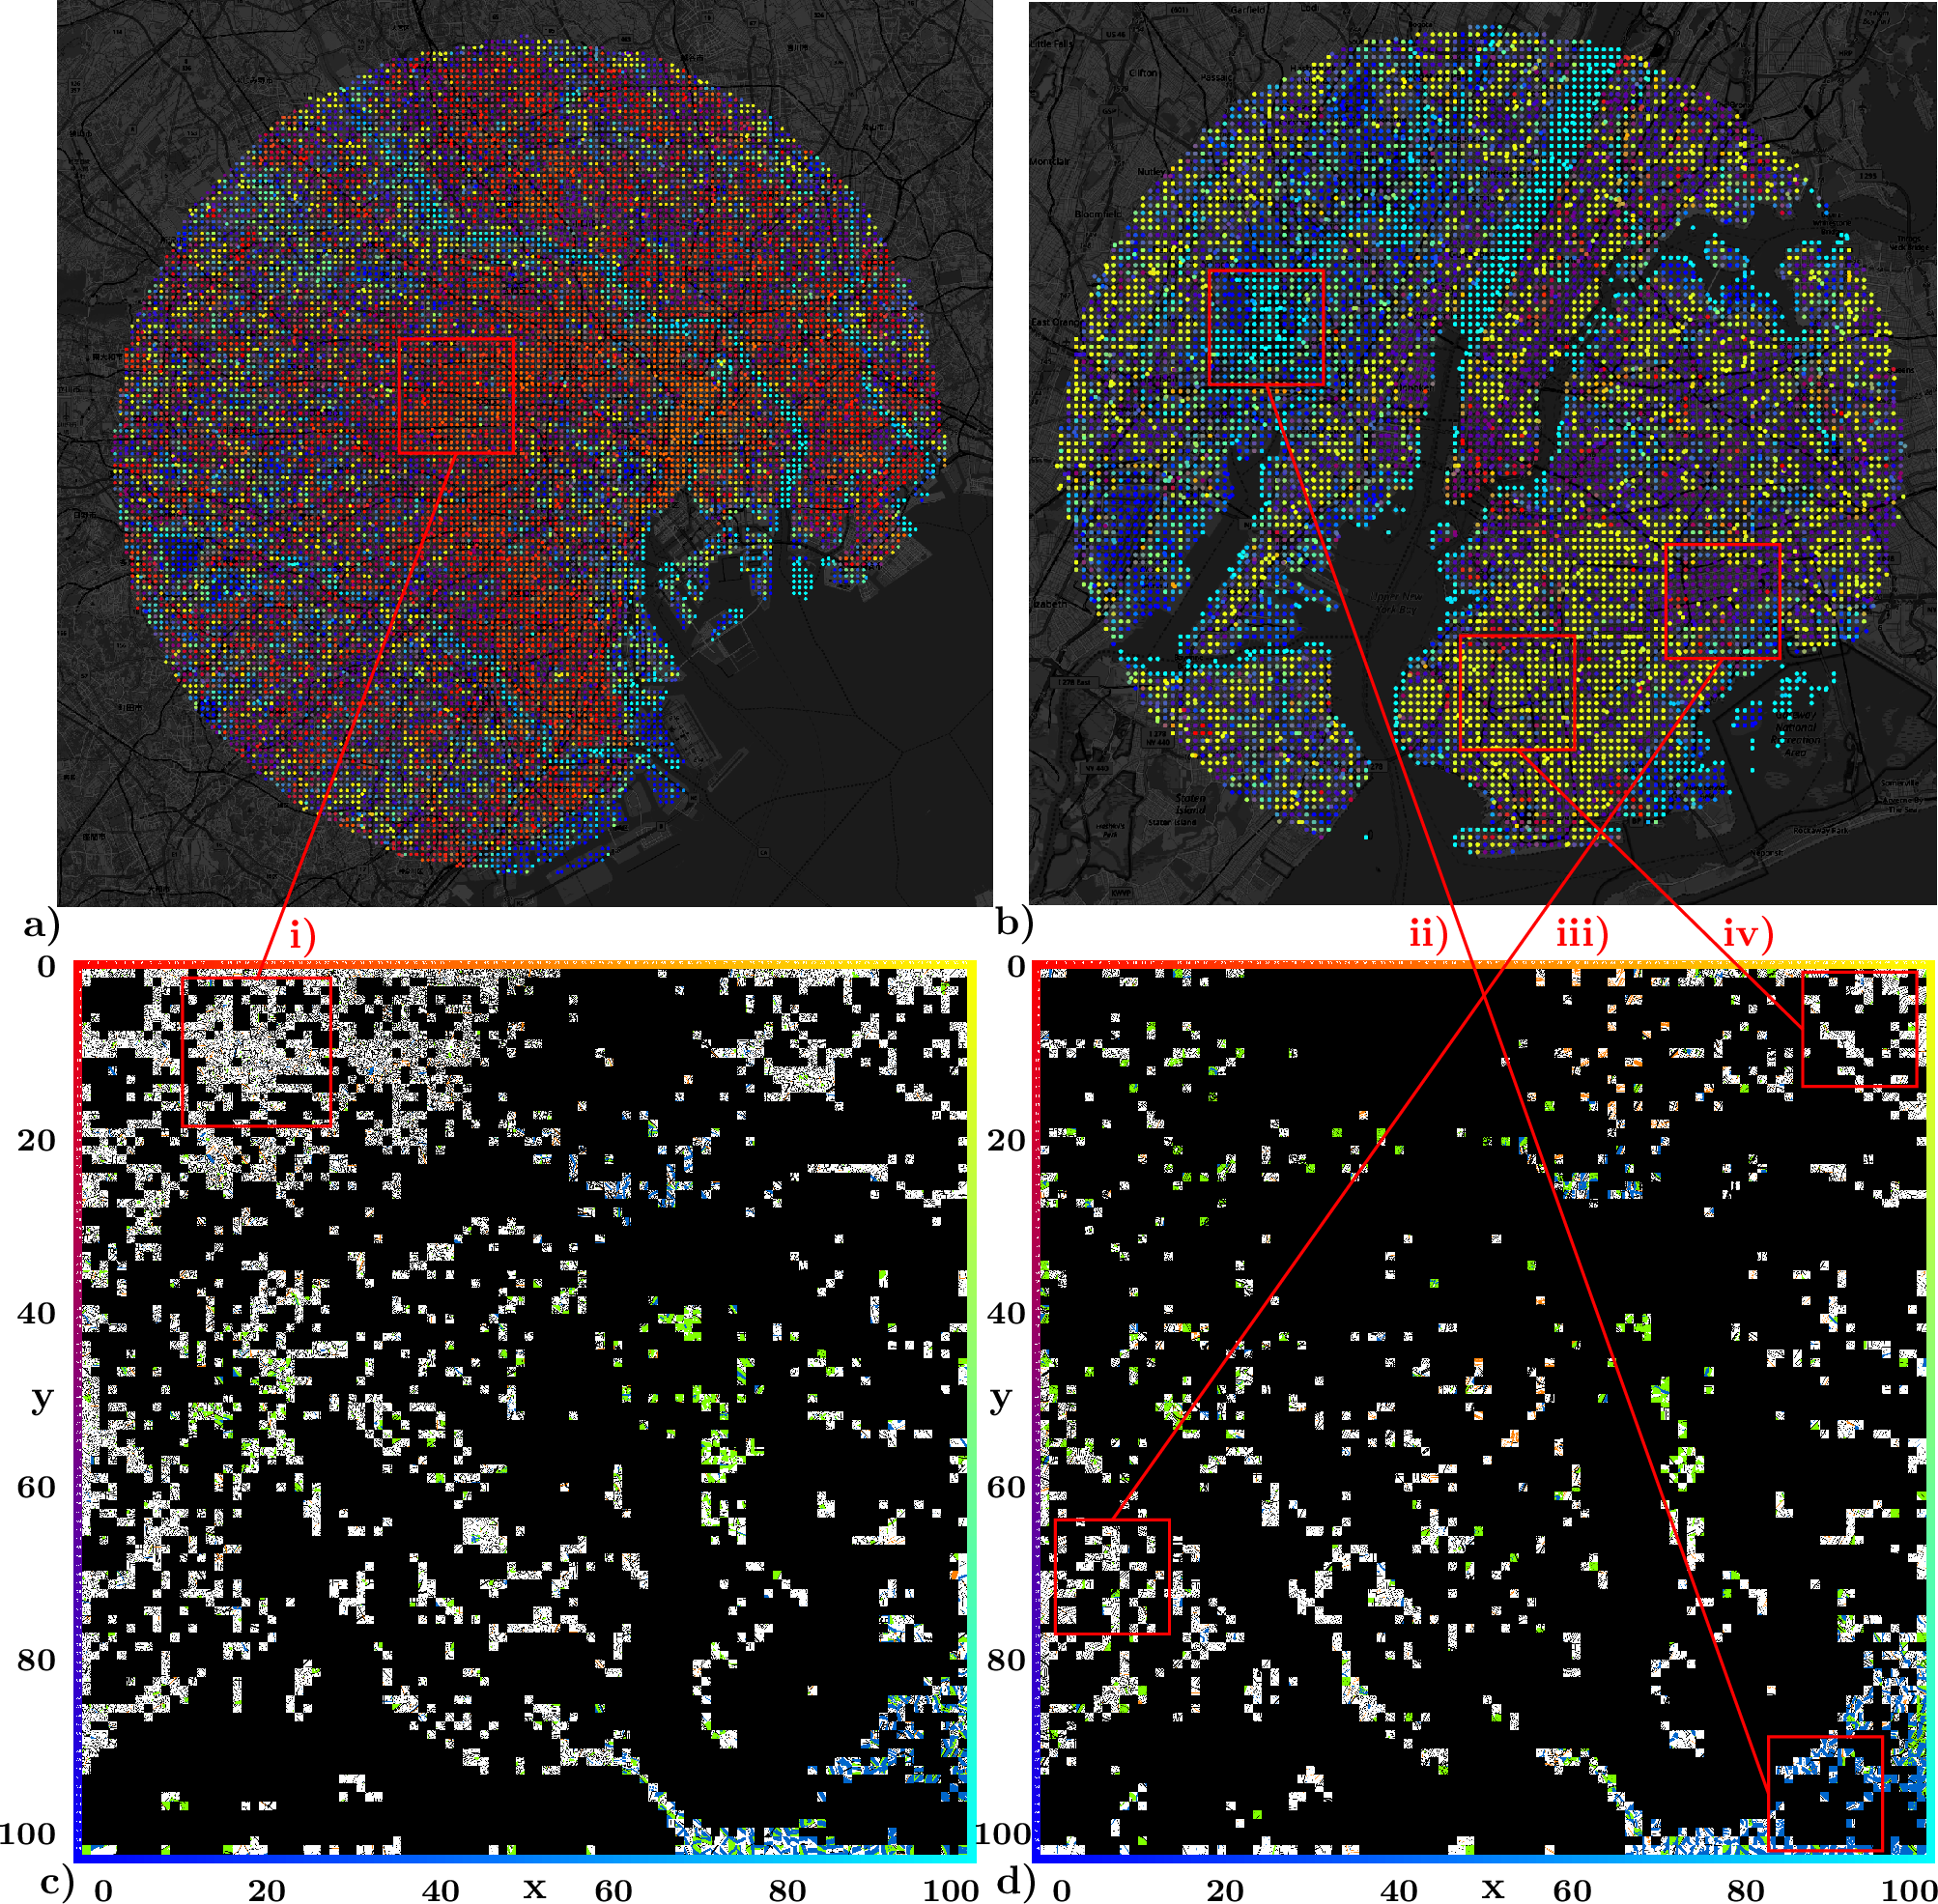
\includegraphics[page=1,trim={58 180 54 188},clip,scale=0.95]{BlockTypologies_Figures5.pdf} 
%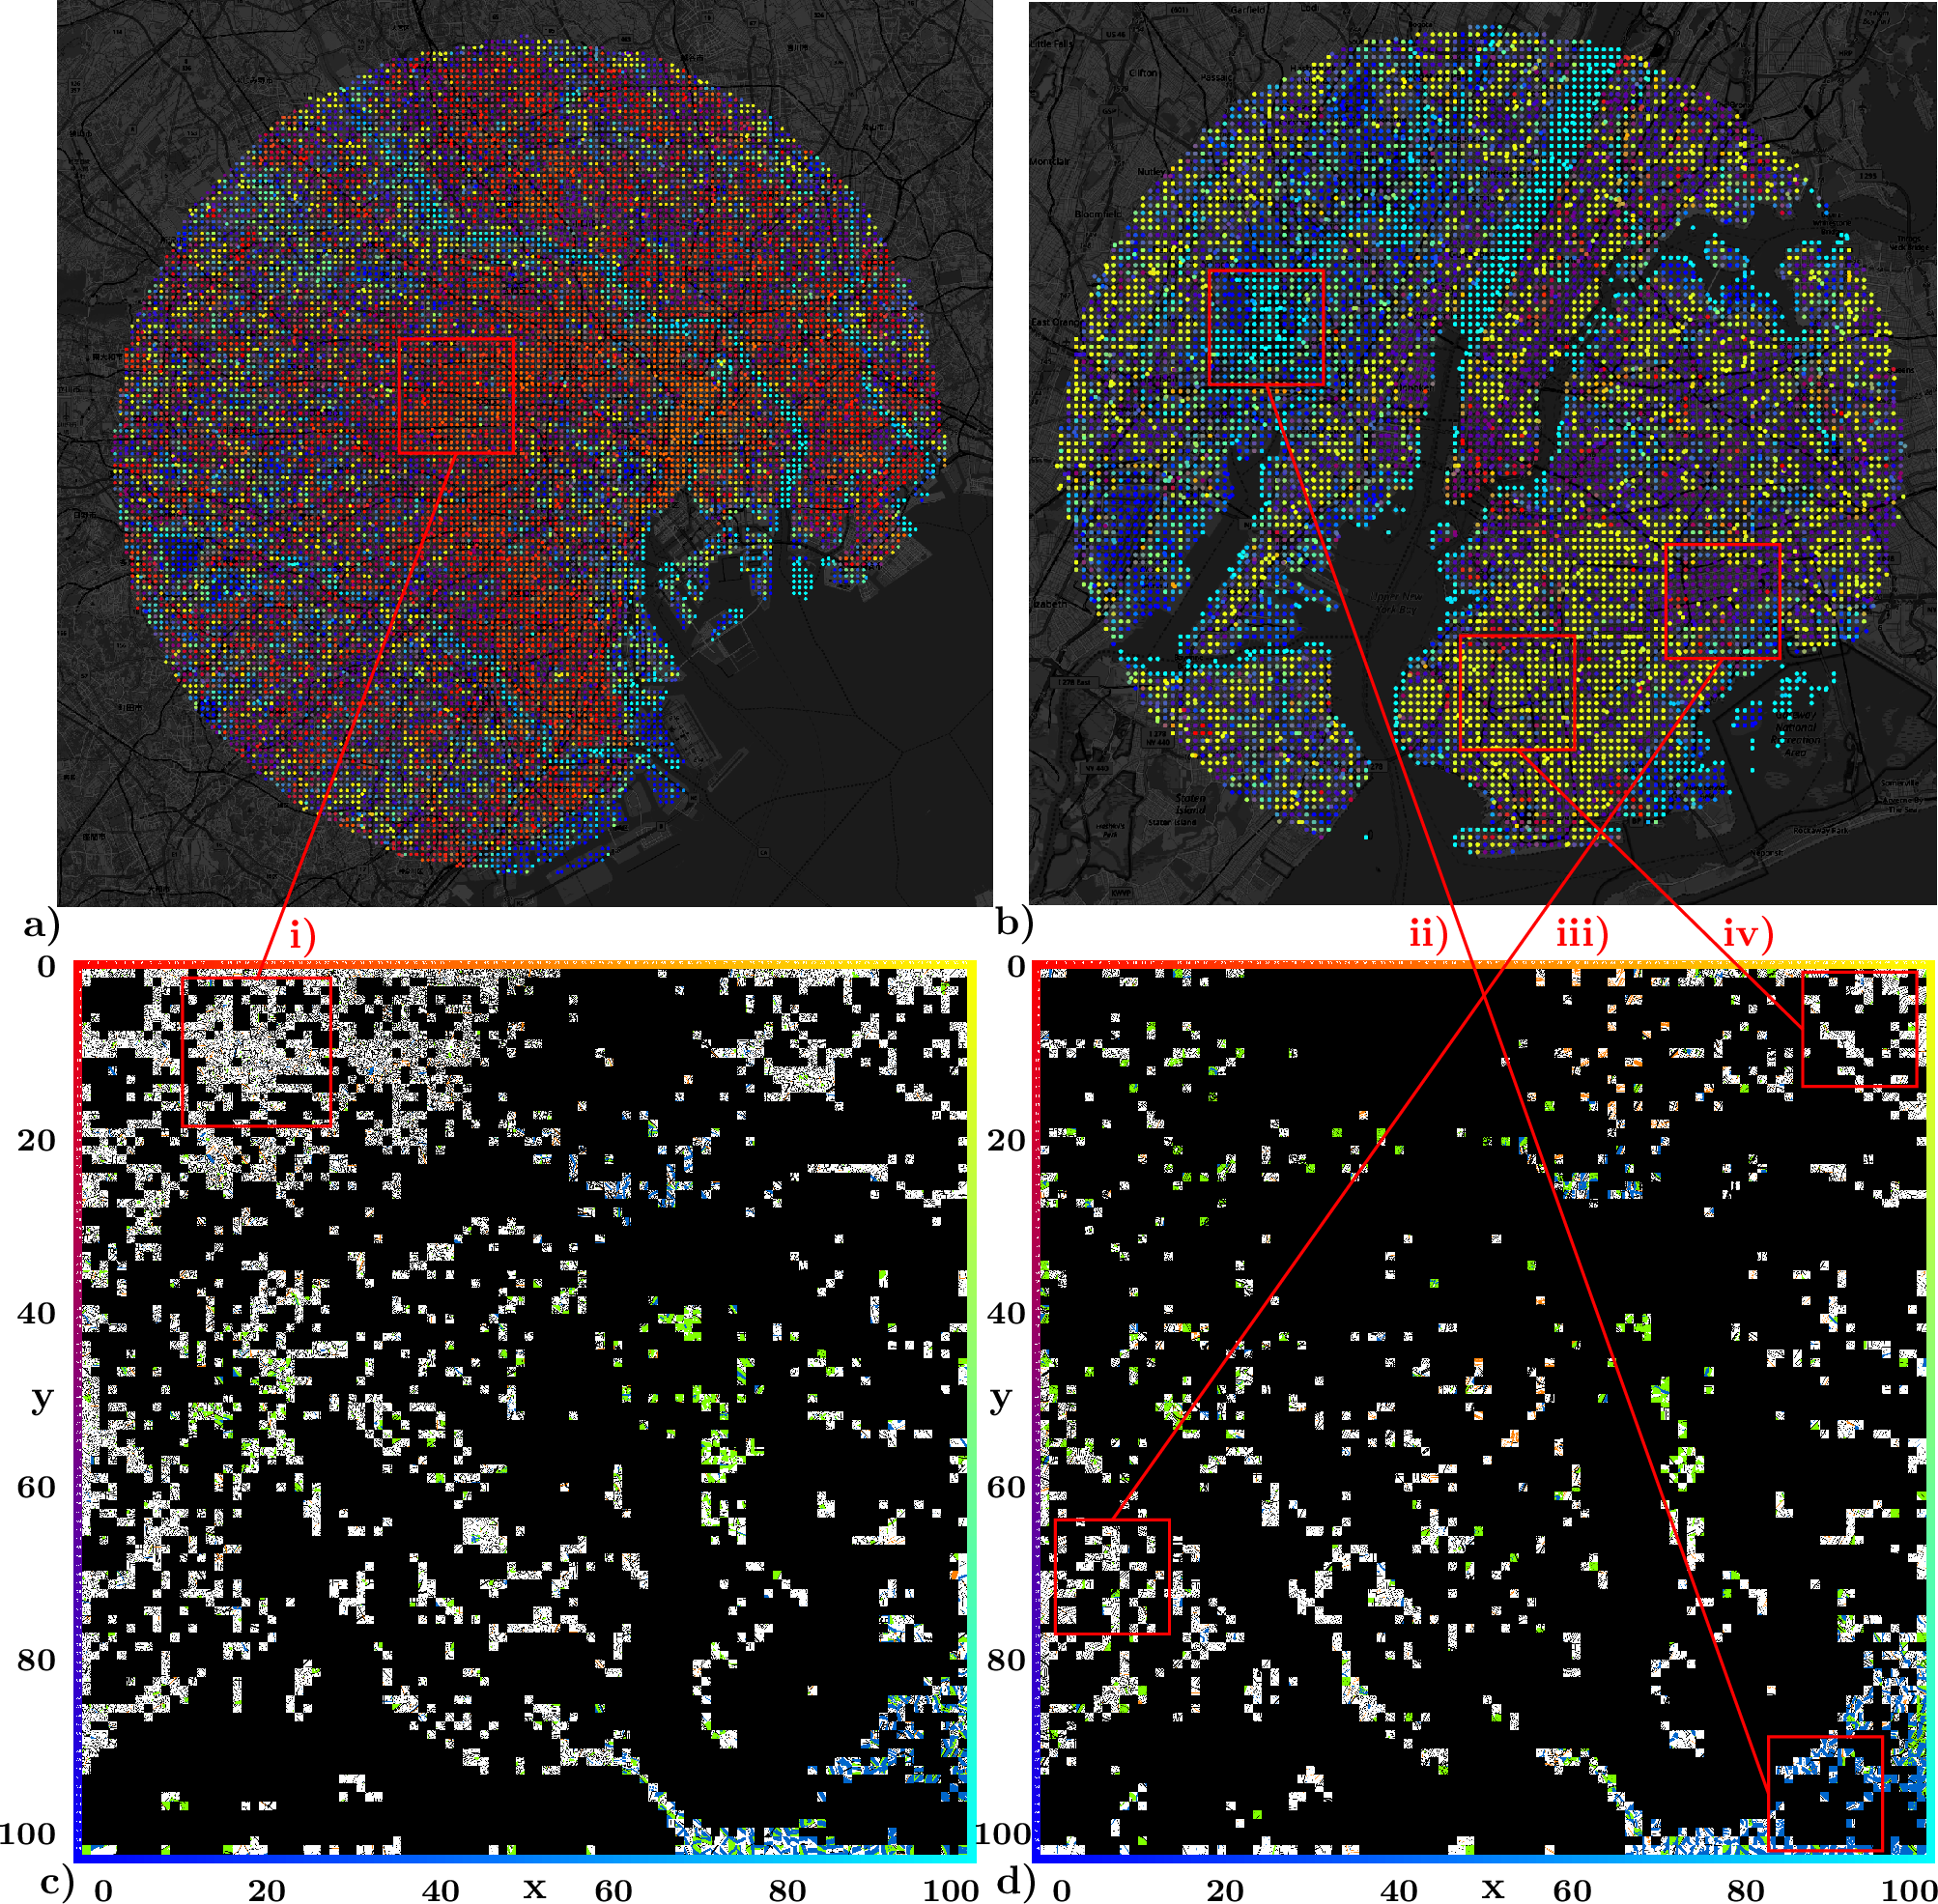
\includegraphics[trim={0 0 0 0},clip,scale=0.12]{BlockTypologies_Figures5.png} 
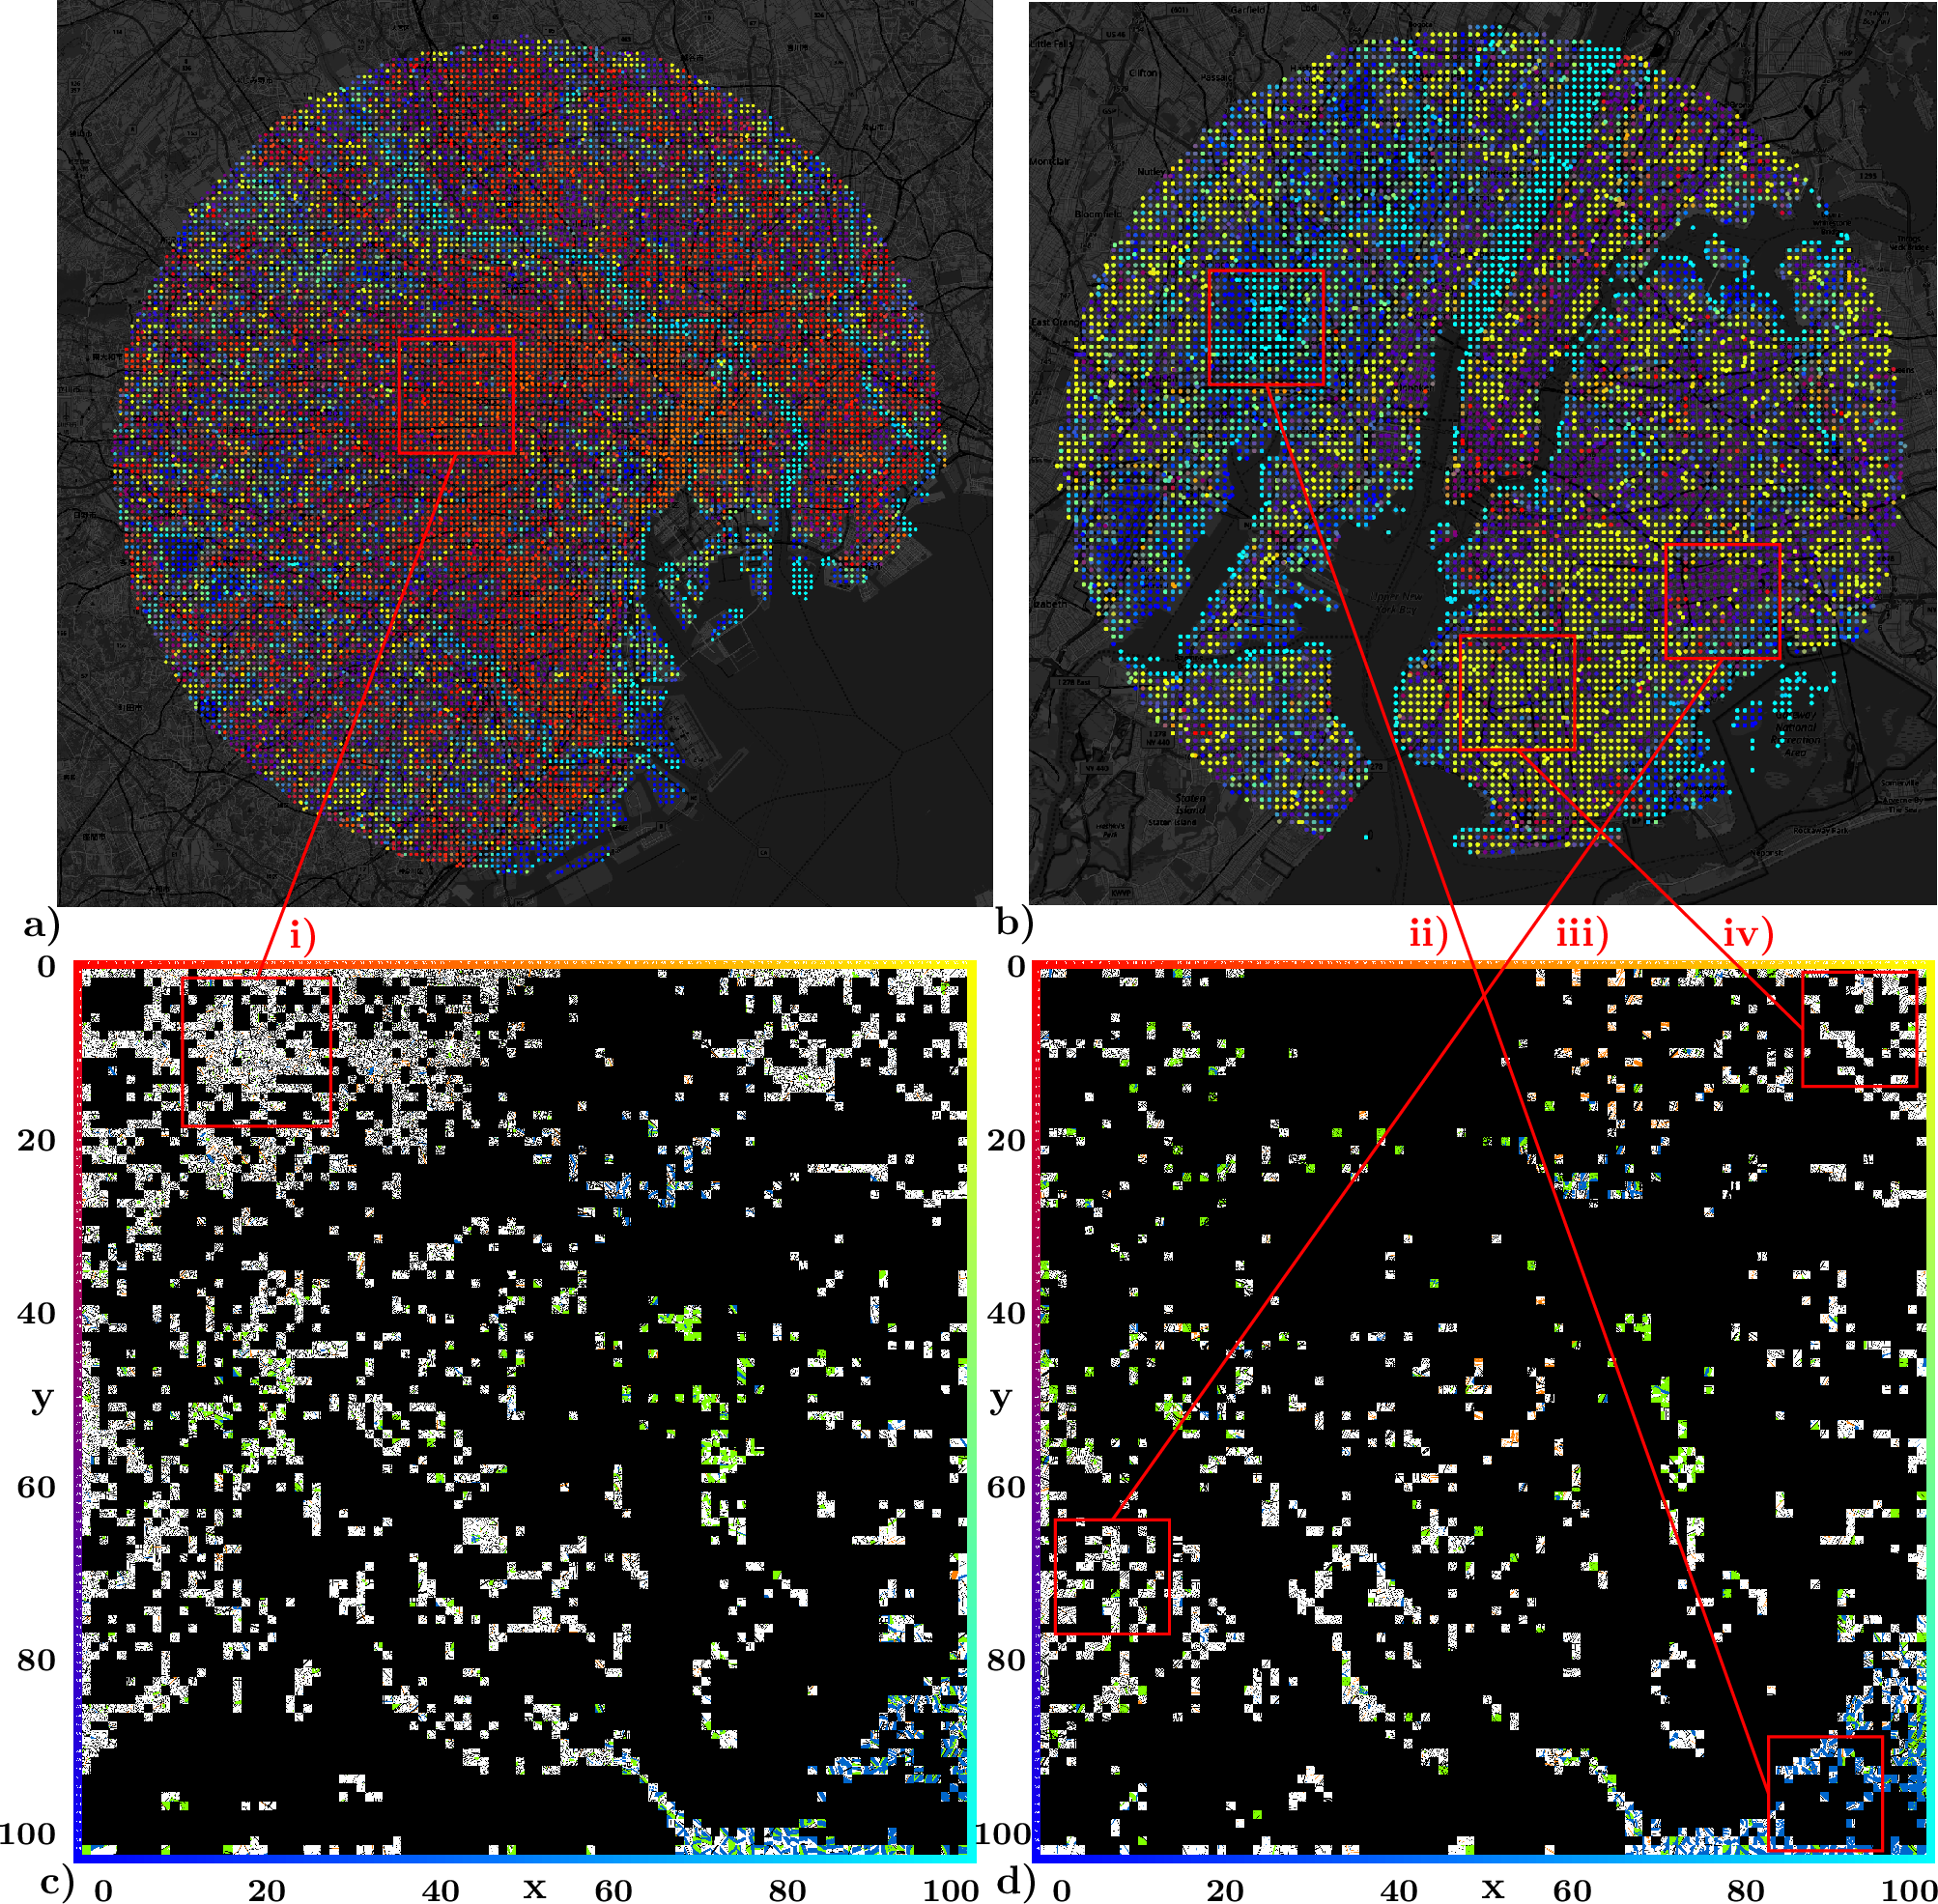
\includegraphics[width=.55\linewidth]{BlockTypologies_Figures5.png}
% }
\caption{\bf Spatial distribution of neighbourhood types (as represented by SOM (x,y) locations) in a) Tokyo and b) New York. City detail maps use the same SOM (x,y) location colour scheme as the border of Figure \ref{fig:somresults} and of Figure \ref{fig:colormap} colour map. SOM visualisation of Figure \ref{fig:somresults} but only displaying locations in c) Tokyo and d) New York. Red boxes and lines i, ii, iii, and iv show neighbourhood types (bottom) corresponding to locations (top) within Tokyo and New York.}
 \label{fig:citylocations}
\end{figure*} 

Using these figures, it can be seen that in Tokyo, neighbourhoods of very small irregular blocks, depicted by the (10,15) orange type (Figure \ref{fig:citylocations} Line i), are concentrated within the inner ring road. In the waterfront areas, a mix of of larger and less structured blocks and mixes of water and green space correspond to the blue and aqua types (SOM areas below the 60 y-axis). The eastern part of the city continues with predominately small irregular blocks while the western side shows a more heterogeneous mix. 

In New York, Brooklyn is predominately large regular gridded blocks (Figure \ref{fig:citylocations} Line iv) depicted by the (98,8) yellow-green types. Queens is a mix of yellow-green types, mixed sized slightly irregular blocks (Figure \ref{fig:citylocations} Line iii) corresponding to (10,70) purple types, and mixed water/green and large blocks (Figure \ref{fig:citylocations} Line ii) of the (85,98) blue type. Purples continue into lower and mid-Manhattan, transforming into a mix similar to Brooklyn in uptown Manhattan and the Bronx. A strip of yellow-green runs north-south down east New Jersey with blue and purple fringes on the water edges.

To validate the application, we calculated mean averages for each (x,y) location (using the 1000 nearest neighbours) in the SOM and the latitude/longitude of those locations using a number of gridded observational datasets of pollution and emissions. We also used a dataset of fractions of classes of urban form, including trees, impervious surfaces, and non-permanent objects (i.e. moving vehicles) calculated from Google Street View at 65 million locations in 70 cities\cite{Middel2019,Middel2018}. Both these datasets enable a validation that block size and regularity can be used to find neighbourhood types reflecting their actual morphology, but also provide insights into how these morphologies reflect transportation infrastructure decisions (allocated road space, amounts of vehicles, and population density) and the impacts of those choices (emissions and air pollution). Figure \ref{fig:meansomresults} shows mean values for the SOM of percentage of a) tree cover and b) impervious surfaces, as well as levels of c) NO$_{2}$, d) population density (from SEDAC dataset), e) Aerosol Optical Depth (AOD), and f) fossil fuel CO$_{2}$ emissions intensity (from FFDAS dataset).

\begin{figure}
\centering
%\includegraphics[page=1,trim={65 295 65 295},clip]{../Article-BlockTypologies/BlockTypologies_Figures4.pdf}
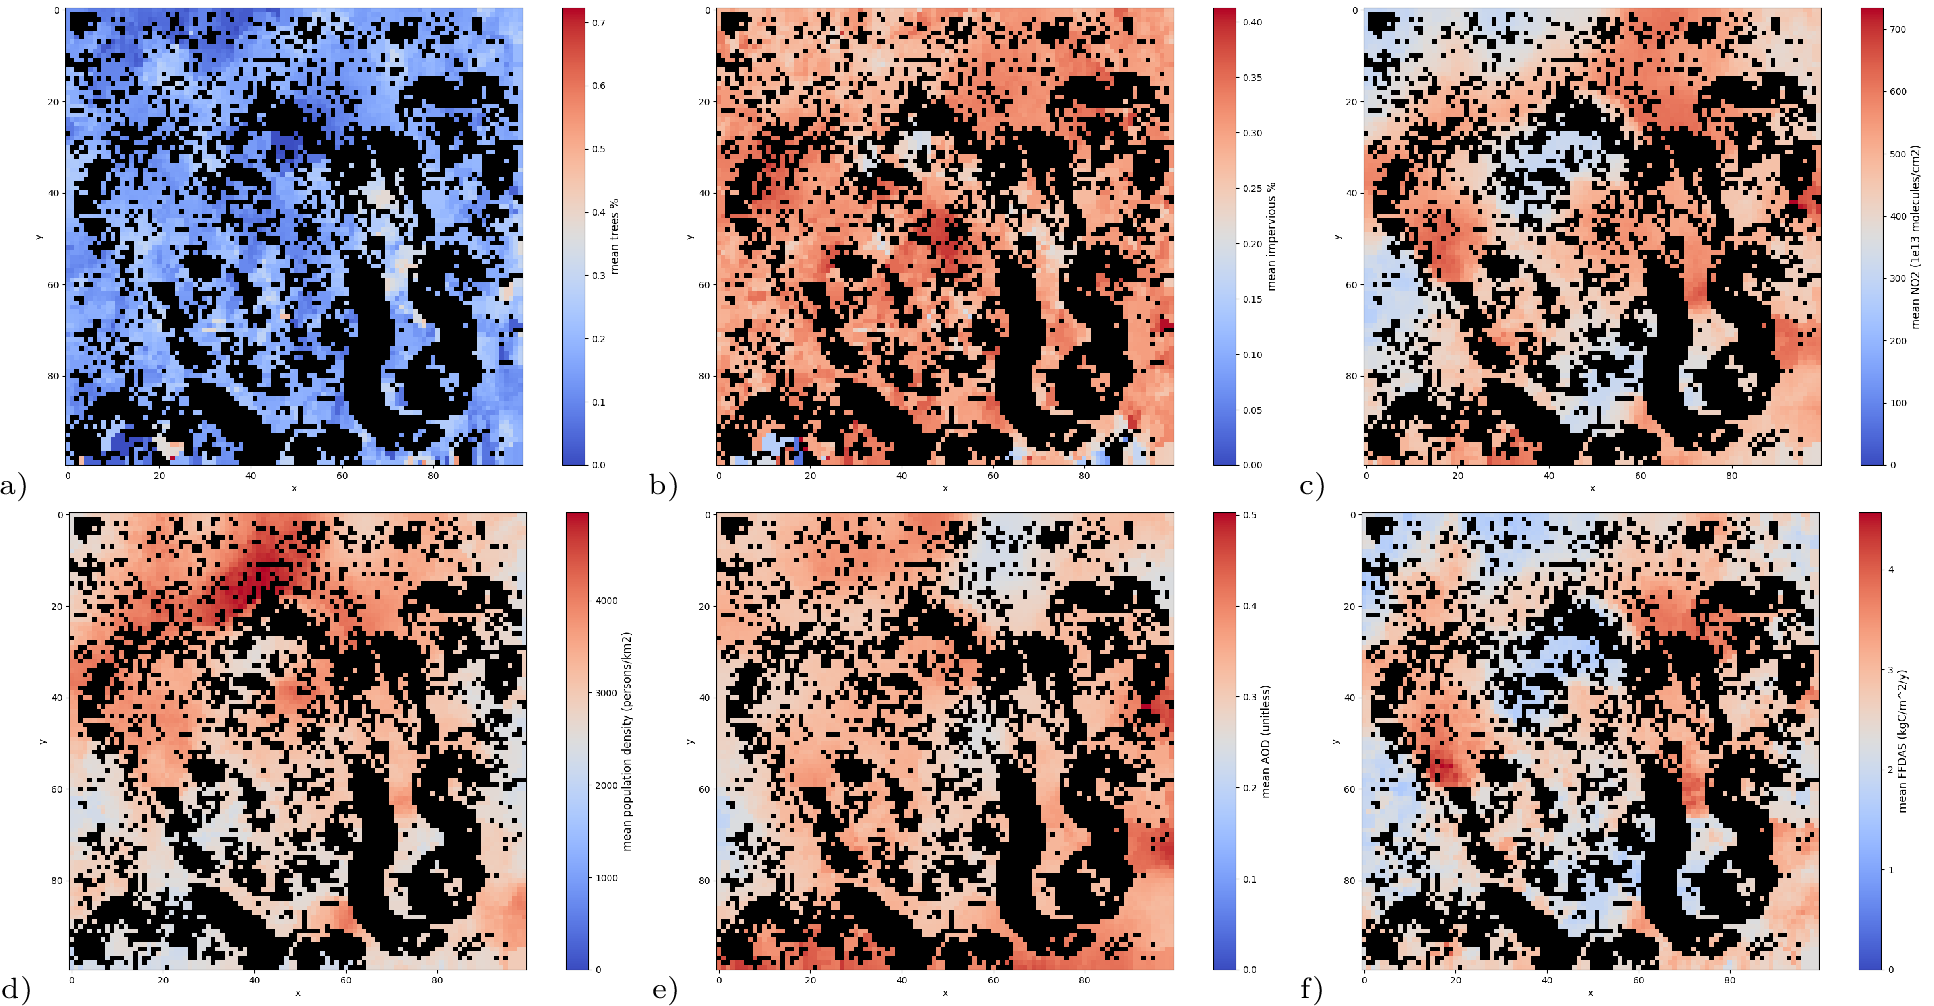
\includegraphics[trim={0 0 0 0},clip,scale=0.14]{BlockTypologies_Figures4-0.png}
\caption{\bf Mean averages for each SOM (x,y) location from Figure \ref{fig:somresults} using the 1000 nearest neighbours. Means calculated using observed values of fractions of a) trees and b) impervious surfaces and values of c) NO$_{2}$, d) population density, e) Aerosol Optical Depth (AOD), and f) fossil fuel CO$_{2}$ emissions intensity (FFDAS).}
 \label{fig:meansomresults}
\end{figure} 

It can be observed in Figure \ref{fig:meansomresults}a, that higher fractions of tree cover correspond to regions in Figure \ref{fig:somresults} with high levels of green space, including (65,40), (22,95), (75,60), and (95,60). In Figure \ref{fig:meansomresults}b, small amounts of impervious surfaces are observed at 95 on the y axis where the map segments show low density streets and areas of high blue space. For population density, Figure \ref{fig:meansomresults}d shows high population density across the (40,20) region where the SOM shows extremely dense street networks and reductions in density moving down the y axis from 60 to 100 where the SOM shows very low density less structured street networks.

While the previous examples (tree cover, surface types, and density) show relationships that can be easily derived from direct observations of urban areas, Figures \ref{fig:meansomresults}c, e, and f show relationships between pollution and urban form that are not possible to observe directly. There are very similar responses to urban form types between NO$_{2}$ and carbon intensity (FFDAS). Areas with high values around (99,40), (20,58), (68,60), and (66,25) correspond to areas with large (often regular) blocks, often combined with a light mix green and blue space. Areas with low values are seen around (45,30), (10,10), (30,5), areas with a very dense mix of and intricate street network and (5,60) and (50,90), areas of slightly less dense street structure. However, AOD often shows a different relationship with urban form than NO$_{2}$ and FFDAS. Where regions around (5,60) show reduced levels of AOD (similar but to a lesser extent to NO$_{2}$ and FFDAS), the areas around (45,30), (10,10), and (30,5) show higher levels of AOD (the inverse of NO$_{2}$ and FFDAS). 

As a further validation, we calculated correlations between mean average values of pollution and elements of urban form for each city compared to averages of weighted averages of the mix of SOM(x,y) locations for each city (Table \ref{table:correlations}). Good correlations are observed for fractions of urban form (ranging from 0.97 to 0.56) as well as good correlations (ranging from 0.58 to 0.57) with pollution levels. Again, these results provide insights into the urban morphological make-up of different cities and transportation decisions underlying each neighbourhood type and the impacts of those choices.

\begin{table}
\centering
\caption{Correlations between mean average values by city and by (x,y) location within the SOM.}\label{table:correlations}
\begin{tabular}{ | c | c |}
\hline \textbf{Parameter} & \textbf{Correlation value}\\ \hline
Movable objects fraction& 0.97 \\ \hline
Impervious surfaces fraction& 0.86 \\ \hline
Sky fraction& 0.75 \\ \hline
Building fraction& 0.56 \\ \hline
Mean AOD& 0.58 \\ \hline
Mean NO$_{2}$&0.57 \\ \hline
\end{tabular}
\end{table}



%\section{Broader Implications}



























%Up to three levels of \textbf{subheading} are permitted. Subheadings should not be numbered.
%
%
%
%\subsection*{Subsection}
%
%Example text under a subsection. Bulleted lists may be used where appropriate, e.g.
%
%\begin{itemize}
%\item First item
%\item Second item
%\end{itemize}
%
%\subsubsection*{Third-level section}
% 
%Topical subheadings are allowed.

\section*{Discussion}

%The Discussion should be succinct and must not contain subheadings.

A look at the range of neighbourhood typologies from individual cities shows that many cities are an eclectic mixture of different neighbourhood typologies but all are built using common elements. An individual city's uniqueness (in this case, the city's structure through its blocks and streets), what we refer to as the city's `fingerprint', is reflected in an individual mix of neighbourhood typologies, with Figure \ref{fig:kernel} showing a number of city `fingerprints' based on the concentration of neighbourhood types. These individual fingerprints can be used to compare cities around the world at a granularity of individual 300$\times$300m neighbourhoods. We find that the uniqueness of cities are derived from a subtle mix of common elements and their spatial distribution (Figure \ref{fig:citylocations}).

\begin{figure}
\centering
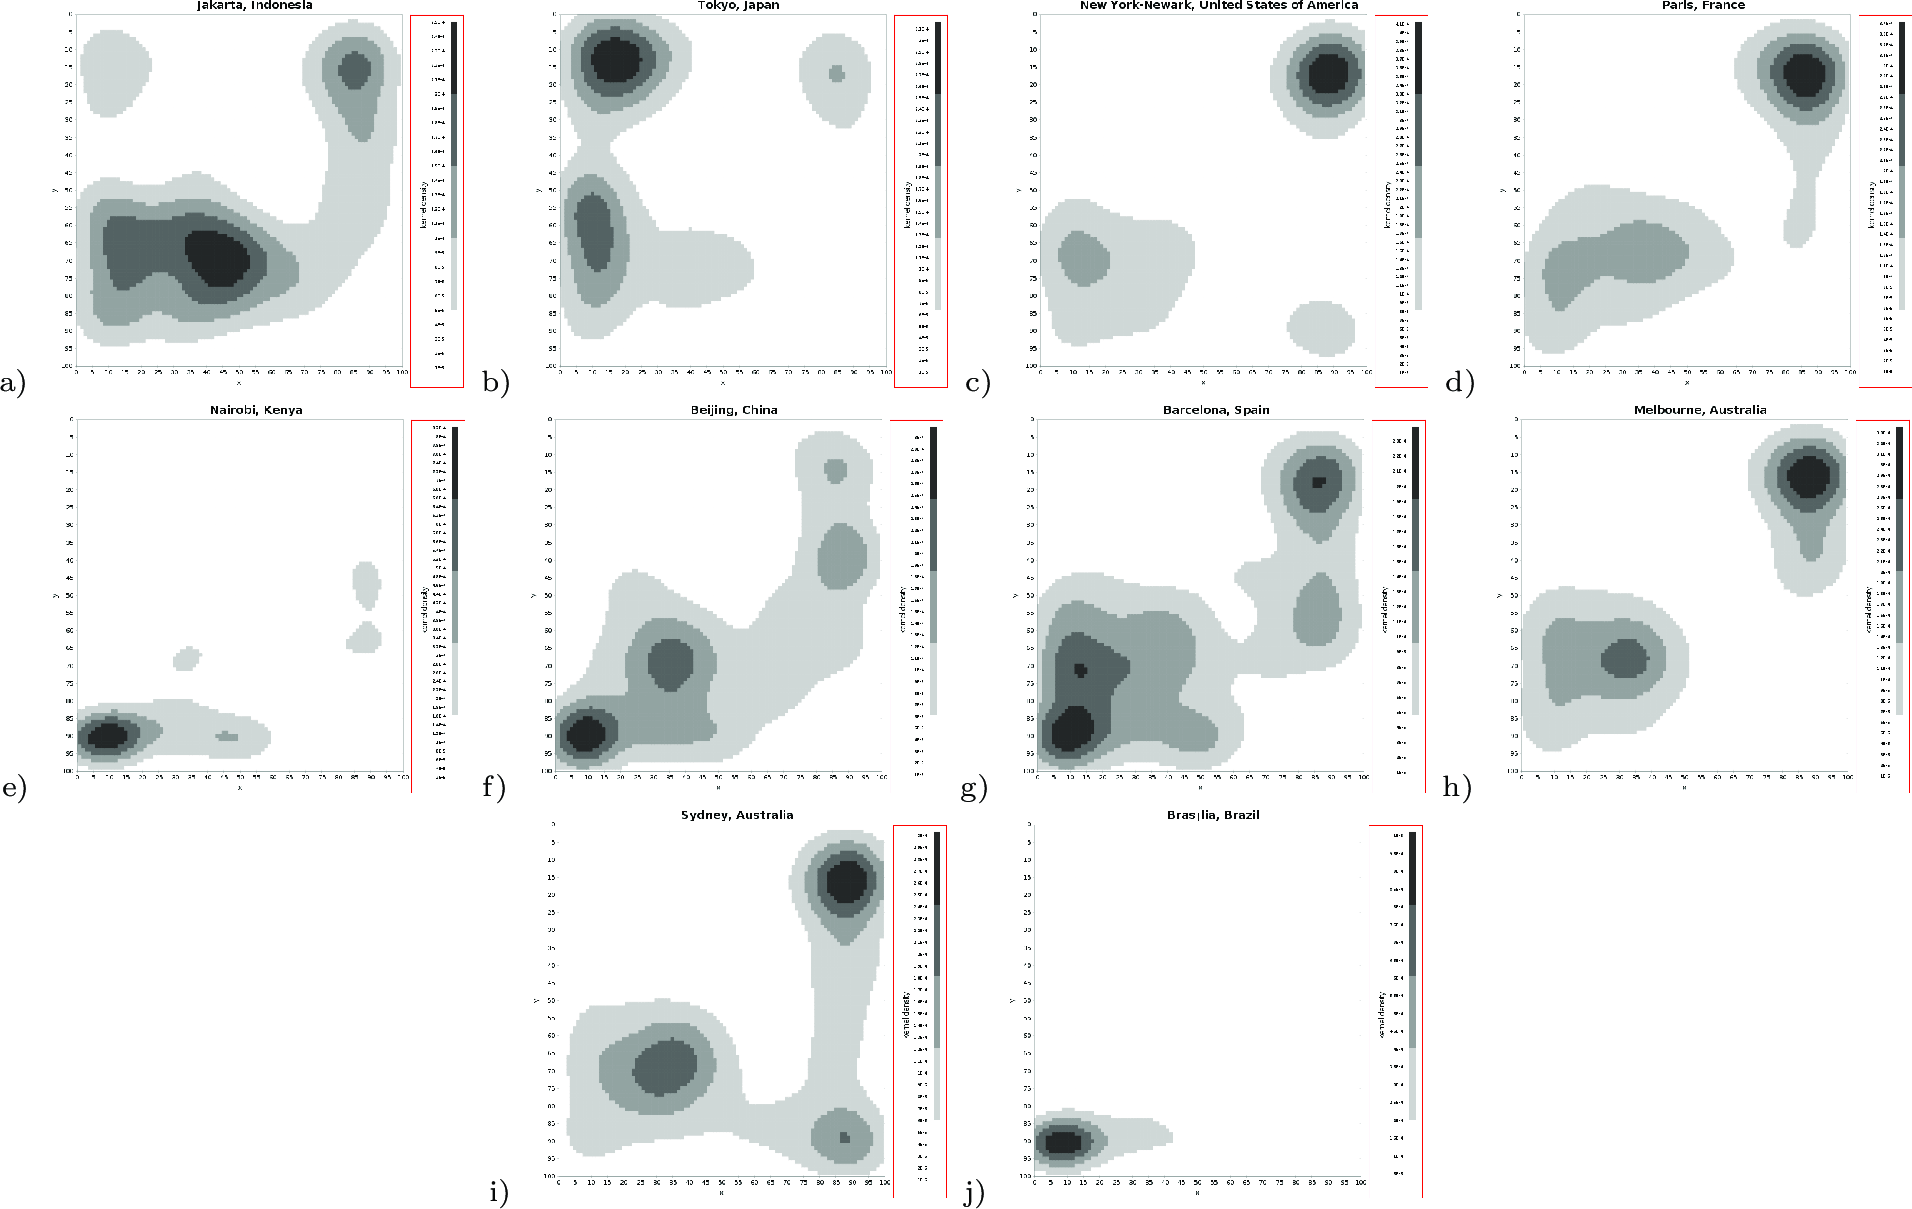
\includegraphics[width=.8\linewidth]{BlockTypologies_Figures2-1.png}
\caption{\bf City fingerprints generated by kernel density maps of SOM (x,y) locations for cities 
a) Jakarta,
b) Tokyo, 
c) New York, 
d) Paris,
e) Nairobi,
f) Beijing, 
g) Barcelona, 
h) Melbourne, 
i) Sydney, and
j) Bras\'{i}lia.
}
 \label{fig:kernel}
\end{figure} 

This provides insights at an unprecedented granularity, uncovering the mix and scale of neighbourhoods across these cities. We have found unique individual neighbourhood types that can have twins in different cities across the globe. We also show the extent to which individual cities are heterogeneous within their bounds and the variation in distribution of neighbourhood types they display. Finally, we show associations between the mixes of neighbourhood typologies derived through our method to both the amounts of different amounts of urban form and the contribution of these neighbourhood typology mixes to measured levels of pollution (as one measure of their performance) in each city. 

Our unique contribution is a method that allows, for the first time, global inter-comparisons of neighbourhoods while highlighting that cities are constructed using fundamental particles; neighbourhood typologies. Due to the stability of the physical structure of cities, undergoing long term small incremental changes\cite{Wegener1986}, this collection represents a collective representation of the built history of human settlements. The implications are both fundamental and practical. It allows improvements to other systems such as health, transportation, and employment that are built on these fundamental components. The system can provide guidance for designers, engineers, stakeholders and policy makers by harnessing insights from a comparison across the globe. 

Our method has highlighted that cities are not unique and that individual neighbourhoods can be compared across continents. The findings also indicate that there is a common structure and that city typologies should be built across cities rather than within, that city centres are more comparable to other centres than to other elements of the same city. It also allows us now to compare cities on a global scale and investigate the nature of human settlements. The link between urban form and vehicle emissions has been shown on an aggregate level\cite{Frank2000}. Similarly, transportation mode choices are associated with block size and accessibility are a primary enabler/inhibitor for residence using active modes of transportation\cite{Ewing2001,Ewing2009a}. As shown in the results, we find strong correlations between different mixes of neighbourhood typologies derived through block size and regularity and the morphology and composition (through fractions of movable vehicles, sky view, buildings and impervious surfaces) of these areas. In addition, we find correlations between the mix of neighbourhood typologies and the performance of the city in terms of pollutants (AOD and NO$_{2}$). This method now allows us to investigate such questions at a neighbourhood scale. 

Finally, in contrast to previous methods which were limited by the available data from a handful of cities, this method is able to span the globe using available globally consistent map data. The method is also extendible and additional variables can be added to the vectors, such as demographic characteristics associated with each location\cite{Kropp1998}, distances to public transport, average building heights, or traffic counts to undercover extra dimensions of associations within the resulting neighbourhood typologies.




























\matmethods
{
%TODO
%Please describe your materials and methods here. This can be more than one paragraph, and may contain subsections and equations as required. Authors should include a statement in the methods section describing how readers will be able to access the data in the paper. 
%}

%\subsection*{Subsection for Method}
%Example text for subsection.
%}




\subsection*{Map imagery sampling}\label{sec:methods2}
The concept employed in this study was to sample maps of individual city sections, calculate block size and regularity of each section, and then use a self organising map (SOM) to organise the images into different urban types. All cities with populations greater than 300,000 people\cite{UN2014} were selected for analysis. Map imagery from Google Maps\cite{GoogleStatic2017} was used to provide globally consistent data. 

A two-stage sampling approach was applied to each city. As no standardised urban boundaries are available for all the cities evaluated in this study, a methodology had to be developed to define these. Firstly, a sampling area extending 1.5 km from the identified city centroid\cite{UN2014} was set as a baseline. Then the sampling radius $r$ (km) was scaled, increasing by a power of 0.85 to the proportional increase in population size based on Barthelemy\cite{Barthelemy2016} in 

\begin{equation}
r = \sqrt{ \frac{28.27}{\pi} \left( \frac{p}{300,000} \right) ^{0.85} }
\end{equation}


Standardising the sampling area in this manner avoided socio-political discrepancies relating to a city's `true' (political) boundary and captured differences in population density and shape between small (e.g., Wellington, New Zealand; Izmit, Turkey) and global mega-cities (e.g., Tokyo, Japan; Delhi, India). Location sampling areas were adjusted for the earth's curvature\cite{Sinnott1984}. Large water-bodies (e.g., oceans but not coastlines) were removed from the sampling area, as they were not indicative of urban form. 

These procedures result in a population and water body-adjusted circular area centred on the city's central coordinates, intended to capture the widest extent of each city while minimising the amount of non-urban locations. For example, Figure \ref{fig:parissample} shows the resulting sampling locations used in collecting imagery for Hong Kong. 

\begin{figure}
\centering
\includegraphics[width=.8\linewidth]{HongKongSamples_.png}
\caption{\bf Sampling locations for map imagery (from Hong Kong).}
 \label{fig:parissample}
\end{figure} 



\subsection*{Map imagery source}\label{methodsimagery}

320$\times$320 pixel sized map images were sampled for 1692 cities using a zoom level of 16 (covering 750$\times$750m at the equator and down to 335$\times$335m at higher latitudes) using a custom style defined with the Google Static Maps API\cite{GoogleStatic2017} (see Figure~\ref{fig:maps} for examples of Paris, France). To ensure each map covers the same area, each image was cropped and resized before processing. The sampled city at the highest latitude was at 64 degrees north, so each image was cropped and resized to include a region of 335$\times$335m. 

The maps provide a high-level abstraction of road (black) and public transport (orange) networks, green space (green), and water bodies (blue). Any remaining space is coded white. Inconsistent map imagery from 25 South Korean cities (due to South Korean government restrictions on map data\cite{Badalge2018}) was removed from the dataset, reducing the number of cities to 1667. 1000 maps were sampled per city. The total dataset consists of nearly 1.7 million images.

\begin{figure}
\centering
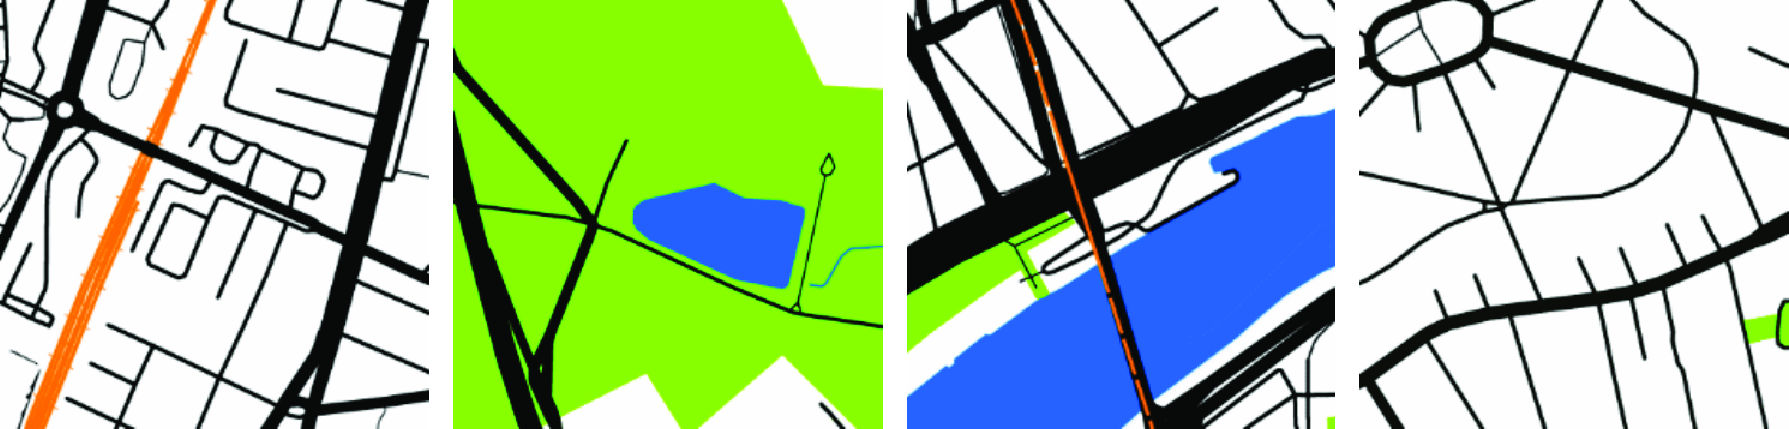
\includegraphics[width=.8\linewidth]{BlockTypologies_Figures2-4.png}
\caption{\bf Four sample Google Maps training data images (from Paris, France)\cite{GoogleStatic2017}.}
 \label{fig:maps}
\end{figure} 

\subsection*{Calculating block size, regularity, and colour counts}\label{methodscalc}

Block size, regularity, and colour counts were calculated for each sampled image with Algorithm \ref{alg:floodfill}, using the Java 8 AWT toolkit\cite{Oracle2018}:

\begin{algorithm}\captionsetup{labelfont={sc,bf}, labelsep=newline}
  \caption{Calculation of histograms of block sizes and regularity}
\begin{algorithmic}
\label{alg:floodfill}
\State Using latitude of image sample, crop the image to represent 335$\times$335 meters
\State Resize image back to 320$\times$320 pixels
\State Start at top left point of image
\While{White pixels are found}
  \State Floodfill area using boundaries of all non-white colours (i.e. black, green, blue, orange)
  \State Count pixel size of region
  \State Construct the smallest bounding box of the cloud of points in the region using the Fast Convex Hull algorithm\cite{Javagl2017,GoogleArchive2011}
  \State Use the difference of counted pixels between the bounding box size and the region size as measure of irregularity
  \State Add size and regularity counts to corresponding (pre-specified) histogram bin
  \State Locate next white pixel by iterating across rows and columns
\EndWhile
\State  Count percentage of blue, orange, green, black, and white pixels in each image
\State  Combine the two size and regularity histograms along with colour counts into a single histogram vector to be used in the SOM
%\Return Histogram of region sizes and region regularity for a single image
\end{algorithmic}
  \hspace*{\algorithmicindent} \textbf{Output:} Histogram of region sizes and region regularity for a single image
\end{algorithm}


Samples of size floodfills and regularity floodfills are shown in Figure \ref{fig:floodfilled}. Sample histograms used in the SOM are shown in Figure \ref{fig:mapsandHist}.

\begin{figure}
\centering
 \includegraphics[width=.8\linewidth]{BlockTypologies_Figures2-5.png}
\caption{\bf Results of flood filled city blocks showing flood fills of each individual region to determine region size (count of pixels in grey). Differences between region size and pixel counts within bounding boxes (outlined in red) are used as a measure of regularity.}
 \label{fig:floodfilled}
\end{figure} 

\subsection*{City size and regularity histograms}\label{methodshist}

Using the calculated counts, two vectors were constructed for each image, one each for block size and block regularity. The vectors were sorted into 15 histogram bins (the number of bins determined by Sturges' formula\cite{Sturges1926}, $\lceil \log_{2}n \rceil +1$, with $n$ being the number of data points). To reduce the clumping of data in the first bin, bins of increasing sizes were used to spread this data across all bins. The first bin starts with a size boundary of 1 and each following bin has a boundary of the current bin boundary times a multiplier. A multiplier of 2.3 was used to fit the maximum count size (320$\times$320 pixels = 102400) into the 15 bins.

The resulting histograms for sample map regions are shown in Figure \ref{fig:mapsandHist}. Histograms input into the SOM were constructed by combining the 15 bins of region size frequencies (on the left side) with the 15 bins of region regularity frequencies (second 15 bins) into a single histogram vector. In addition, the 5 colour pixel percentages are appended to the end of the histogram vector. Finally, the vector values are normalised into a range of 0 to 1.


\begin{figure}
\centering
 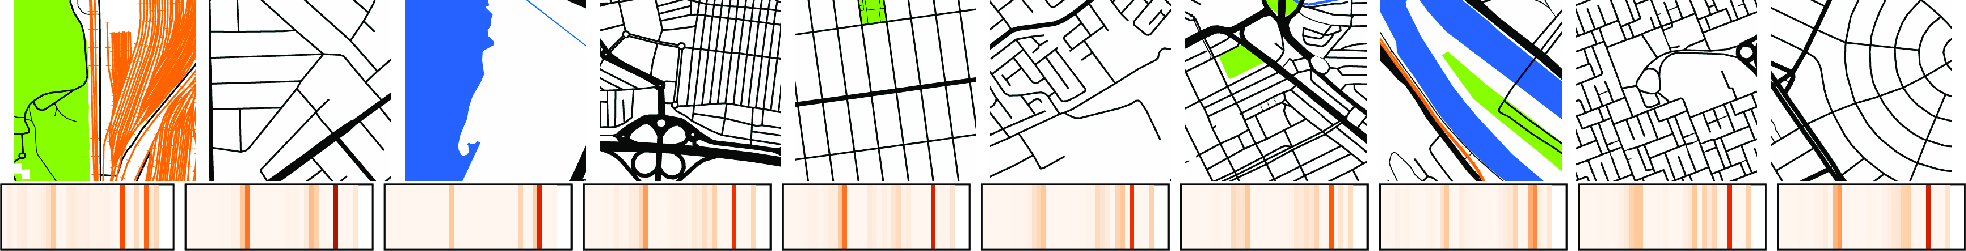
\includegraphics[width=.8\linewidth]{BlockTypologies_Figures2-6.png}
\caption{\bf Samples of map regions (top) and resulting histograms (bottom). Region size, regularity, and colour counts are joined into a combined histogram vector, with size frequencies in the first 15 bins, regularity in the second 15 bins and colour pixel counts in the remaining 5 bins.}
 \label{fig:mapsandHist}
\end{figure} 

\subsection*{Sorting map histograms in the self organising map}\label{methodscluster}
The SOM methodology\cite{Kohonen1982} is a data driven technique that transforms a multi-dimensional data source into a lower dimensional space, commonly a two-dimensional map, while keeping the relative proximity of two datapoints intact. The distance in the lower dimensional representation is therefore a similarity index, calculated as the euclidean distance, of the higher dimensional space. Each point in the two-dimensional map has location (x,y) and is associated with a vector of values from the multi-dimensional space.

SOM is a generic, objective and robust methodology that has been deployed in many domains and is used for the visualisation of multi-dimensional data and data exploration\cite{Koleheimen2004}. This methodology was chosen for its ability to create two-dimensional maps of smoothly changing patterns from the original high-dimensional space. Additionally, the SOM map spans the extremes observed in the original data and allows for investigation on how the data is distributed, potential paths between two observations. 

The 1.7 million map histograms with 35 dimensions were the initial data space used to train the two-dimensional SOM. After the randomised initialisation of the 100x100 nodes of the SOM, a random selection of 5.4 million data points from the initial data space were used to transform the two-dimensional SOM to match it. This iterative process locates nodes that are similar to the training vector and morphs the values of the SOM nodes towards the training values. The number of iterations were determined by the minimum number of iterations to reach the greatest continuity among clusters. Training was stopped when the clusters started becoming discontinuous, checking every 150,000 iterations for a rapid increase in number of clusters. However, experimentally, we found that once a sufficient number of iterations were run, subsequent iterations only had small impacts on the results. 

This training is subjugated to a decay function for both magnitude (learning decay, $L_{i}$) and distance (radius decay, $D_{R}$) in the SOM. Radius decay was calculated using

\begin{equation} 
D_{R} = r_{0} e^{-\frac{i}{n} \log _{10} (r_{0})}
\end{equation}
where radius ($r_{0}$) is 50 (the width and height of the SOM was 100) and the current training iteration $i$ (of total iterations $n$ of 3.2 million). Learning decay is calculated as
\begin{equation} 
L_{i} = L_{0} e^{-\frac{i}{n}}
\end{equation}
where learn rate ($L_{0}$) = 0.05.

After the SOM was trained, each map histogram was classified to find the closest matching node in the SOM. The underlying imagery of the resulting trained SOM was visualised by tiling representative map images from each node (x,y) point in the SOM in Figure \ref{fig:somresults}. Areas with black have no associated map segments with that particular node's (x,y) location (about 5000 nodes). Most nodes are associated with multiple map segments that have similar characteristics. One notable outlier exists that accumulates more than 60,000 map segments of (0,99) with 385,967 maps that are all or nearly all white. Approximately 20 nodes contain 60,000 to 10,000 maps, about 200 contain 10,000 to 1000 maps, 5700 nodes contain 1000 to 1 map.

%0	99	385967
%99	8	58542
%46	99	50585


The node's (x,y) locations were encoded into RGB colour codes using a Java 8 port of Color2D\cite{Jackle2017,Steiger2015}. These colours were used in plotting the (x,y) typologies in QGIS\cite{QGIS2009}.


\subsection*{KernelDensityEstimator2D}\label{kerneldensity}

To create the city fingerprints, kernel density plots were made of the SOM x,y locations for each city using the KernelDensityEstimator2D (a bi-variate kernel density smoother for data) module from the Bayesian Evolutionary Analysis by Sampling Trees (BEAST) software package \cite{Suchard2018} with a smoothed grid size of 100.

% KernelDensityEstimator2D kde = new KernelDensityEstimator2D(dataXa, dataYa, null, 100, null); // 100 is smoothed grid size

\subsection*{Aerosol Optical Depth (AOD) Dataset}\label{aod}
Two near-identical MODIS (Moderate Resolution Imaging Spectroradiometer) instruments are mounted upon the sun-synchronous polar-orbiting NASA satellites Terra and Aqua; these missions have over-pass times of approximately 10:30am and 1:30pm local time and were launched in 1999 and 2004, respectively. The MODIS resolution is 10 km $\times$ 10 km at nadir. The MOD04 and MYD04 L2 retrievals (V006) were downloaded and gridded to 0.05$^\circ$ x 0.05$^\circ$ (grid-spacing of approximately 5.6km). A range of different retrievable fields are available of which we used "Optical\_Depth\_Land\_And\_Ocean" (see Table B1 of Levy et al. (2013)\cite{Levy2013}), which represents a compromise between quality and coverage. These data were averaged to a monthly temporal resolution on this grid, and the number of MODIS pixels contributing to each averaged value were recorded. At each grid-point, a time-series decomposition into seasonal, trend and irregular (STL) components was applied\cite{Cleveland1990}. A slight modification to the code of the STL algorithm in the R stats package\cite{RCoreTeam2015} was made so that data were weighted by the number of observations involved in creating these observations. The trend component is estimated as a smooth function (via the locally weighted scatterplot smoothing, or LOESS, algorithm of Cleveland et al. (1992)\cite{Cleveland1992}), however the trend window parameter (defining the smoothing length scale for the trend term) was set sufficiently high that this term was effectively a linear term. From this, we derived the mean concentration at each grid-point accounting for long-term trend and seasonal fluctuations.

\subsection*{NO$_{2}$ Dataset}\label{no2}
The tropospheric-column NO$_{2}$ data were derived from the TEMIS (Tropospheric Emission Monitoring Internet Service) OMI (Ozone Monitoring Instrument) tropospheric-column NO$_{2}$ (tcNO$_{2}$) database\cite{Boersma2007a}. Monthly gridded averages at 0.125$^\circ$ $\times$ 0.125$^\circ$ resolution (a grid-spacing of roughly 13km) were downloaded from the TEMIS website. These are based on the Level-2 tropospheric-column retrievals. While this provides little vertical information, the tcNO$_{2}$ product shows a good correlation with surface NO$_{2}$ concentrations, when averaged over a sufficient period. The OMI is mounted aboard NASA's sun-synchronous, polar-orbiting satellite Aura (launched July 2004). In normal operation, the OMI pixels are 13 km $\times$ 24 km at their finest (i.e. at nadir). The combination of the instruments wide swath (spanning about 2600 km) and the 14 orbits daily provides a global coverage every day, however retrievals are not possible everywhere, mainly due to clouds. Airborne aerosols and surface albedo are other significant sources of uncertainty. The monthly tcNO$_{2}$ data from 2005-2016 (complete years) were averaged at their native resolution.

\subsection*{City fractions dataset}\label{gsvdata}
Middel et al. (2019,2018)\cite{Middel2019,Middel2018} derived fractional breakdowns from Google Street View (GSV) panorama images for 65 million locations across 75 cities of six urban form classes of sky, trees, buildings, impervious surfaces, pervious surfaces, and non-permanent objects (i.e. moving vehicles). Data for each location was indexed by city, latitude, and longitude. 

\subsection*{Carbon intensity (FFDAS) dataset}\label{ffdasdata}
Rayner et al. (2010)\cite{Rayner2010a,Asefi-Najafabad2014} produced a high-resolution, global quantification of fossil fuel CO$_{2}$ emissions with their fossil fuel data assimilation system (FFDAS). We retrieved their gridded NetCDF yearly totals for 2010 (the latest year of this dataset) which provide values of $kgC/m^{2}/year$ at a 0.1$^\circ$ resolution. The quantified carbon sources include electricity generation and all other fossil fuel emissions (excluding shipping and aviation).

\subsection*{SEDAC population density dataset}\label{populationdata}
The Gridded Population of the World, Version 4 (GPWv4) data collection\cite{CIESIN2018} from The Socioeconomic Data and Applications Center (SEDAC) was used to provide observations of population density. This provides global measures of population density at a resolution of 2.5 arc minutes (about 0.0416$^\circ$ or approximately 5km).

\subsection*{Nearest neighbour averages}\label{knndata}
For each (x,y) point in the SOM, the groupings of (x,y) points required to include the 1000 nearest neighbours were calculated using the Euclidean Distance method from the Apache Commons Math library\cite{ApacheCommons2019}. Then for each point, these groupings were used to calculate mean values for each (x,y) point using the various observation datasets. (x,y) locations without associated map segments were assigned a value of NaN. The results were plotted on contour plots.

\subsection*{City correlations}\label{correlations}
Mean averages for each city were generated using the same centroid area as in the "Map imagery sampling" section above, however locations were sampled at a 400$\times$400m resolution instead of the 1000 randomly selected locations. Using these locations, mean values of AOD and NO$_{2}$ were calculated for 1667 cities. A second set of city mean values were generated for 34 cities that matched the cities sampled for this study using the city fractions dataset.

Next, mean averages of pollution (AOD and NO$_{2}$) and of urban form fractions were calculated for each SOM(x,y) location. The latitude and longitude of each point (for the 1.7 million points) was used to look up an individual value from the gridded pollution datasets. For the city fractions dataset, latitude and longitude locations were matched to 0.0001 degree, for a total of approximately 8500 locations.

Finally, mean averages were calculated using the SOM(x,y) averages for the 1000 locations for 1667 and 34 cities for pollution and urban form respectively. Then the cor() function, using "pairwise.complete.obs" and "pearson", from the R stats package\cite{RCoreTeam2015} was used to find correlations between the two sets of computed city averages for the pollution and city fractions datasets.

\subsection*{Code availability and licensing}\label{sec:available}
Code and data are available from the corresponding author on request and are distributed under the Creative Commons Attribution-NonCommercial-ShareAlike 4.0 Generic (CC BY-NC-SA 4.0) license.
%Also, data and code are available at 
%https://doi.org/10.5281/zenodo.2562396 and https://bitbucket.org/politemadness/skypixeldetection \citep{Nice2019SkyCode} and are distributed under the Creative Commons Attribution-NonCommercial-ShareAlike 4.0 Generic (CC BY-NC-SA 4.0) license. 







} % end of methods







\showmatmethods{} % Display the Materials and Methods section

\acknow{Please include your acknowledgments here, set in a single paragraph. Please do not include any acknowledgments in the Supporting Information, or anywhere else in the manuscript.}

%\showacknow{} % Display the acknowledgments section

% Bibliography
\bibliography{shortbib}

\end{document}
